%%%%%%%%%%%%%%%%%%%%%%%%%%%%%%%%%%%%%%%%%%%%%%%%%%%%%%%%%%%%%%%%%%%%%%%%%%%%%%%%
%2345678901234567890123456789012345678901234567890123456789012345678901234567890
%        1         2         3         4         5         6         7         8

\documentclass[letterpaper, 10 pt, conference]{ieeeconf}  % Comment this line out if you need a4paper

%\documentclass[a4paper, 10pt, conference]{ieeeconf}      % Use this line for a4 paper

\IEEEoverridecommandlockouts                              % This command is only needed if 
                                                          % you want to use the \thanks command

\overrideIEEEmargins                                      % Needed to meet printer requirements.

% See the \addtolength command later in the file to balance the column lengths
% on the last page of the document

% The following packages can be found on http:\\www.ctan.org
\usepackage{graphicx}
\usepackage{graphics} % for pdf, bitmapped graphics files
\usepackage{epsfig} % for postscript graphics files
\usepackage{subcaption}
%\usepackage{mathptmx} % assumes new font selection scheme installed
%\usepackage{times} % assumes new font selection scheme installed
\usepackage{amsmath,amssymb,amsfonts} % assumes amsmath package installed
%\usepackage{booktabs}

% format for theorems etc.
\newtheorem{thm}{Theorem}
\newtheorem{lem}{Lemma}
\newtheorem{cor}{Corollary}
\newtheorem{prop}{Proposition}
\newtheorem{rem}{\bfseries Remark}

% format for argmin, argmax
\newcommand{\argmax}{\operatornamewithlimits{argmax}}

% format for cross-reference
\usepackage[capitalize]{cleveref}
\crefname{equation}{}{}
\Crefname{equation}{Eqn.}{Eqn.}
\crefname{thm}{theorem}{theorems}
\Crefname{thm}{Theorem}{Theorems}
\crefname{lem}{lemma}{lemmas}
\Crefname{lem}{Lemma}{Lemmas}
\crefname{cor}{corollary}{corollaries}
\Crefname{cor}{Corollary}{Corollaries}
\crefname{prop}{proposition}{propositions}
\Crefname{prop}{Proposition}{Propositions}
\crefname{rem}{remark}{remarks}
\Crefname{rem}{Remark}{Remarks}

%=====todonotes===== %
\usepackage{todonotes}
\usepackage{soul}
\definecolor{smoothgreen}{rgb}{0.7,1,0.7}
\sethlcolor{smoothgreen}

\newcommand{\todopara}[1]{\vspace{0px} %
	\todo[inline, color=black!10]{\textbf{[Paragraph:]} {#1}} %
}
\newcommand{\todonote}[1]{\vspace{0px} %
	\todo[inline, color=green!30]{\textbf{[Note:]} {#1}} %
}
\newcommand{\todoQ}[1]{\vspace{0px} %
	\todo[inline, color=orange!50]{\textbf{[Note:]} {#1}} %
}
\newcommand{\todohere}[1]{\hl{(\textbf{TODO:} #1)}}

\newcommand{\hidetodos}{
	\renewcommand{\todopara}[1]{}
	\renewcommand{\todonote}[1]{}
	\renewcommand{\todoQ}[1]{}
	\renewcommand{\todohere}[1]{}}


\title{\LARGE \bf
Distributed Bayesian Filter for Multi-Robot Network by Using Local-Exchange-of-Observation Strategy}


\author{Albert Author$^{1}$ and Bernard D. Researcher$^{2}$% <-this % stops a space
\thanks{*This work was not supported by any organization}% <-this % stops a space
\thanks{$^{1}$Albert Author is with Faculty of Electrical Engineering, Mathematics and Computer Science,
        University of Twente, 7500 AE Enschede, The Netherlands
        {\tt\small albert.author@papercept.net}}%
\thanks{$^{2}$Bernard D. Researcheris with the Department of Electrical Engineering, Wright State University,
        Dayton, OH 45435, USA
        {\tt\small b.d.researcher@ieee.org}}%
}


\begin{document}



\maketitle
\thispagestyle{empty}
\pagestyle{empty}


%%%%%%%%%%%%%%%%%%%%%%%%%%%%%%%%%%%%%%%%%%%%%%%%%%%%%%%%%%%%%%%%%%%%%%%%%%%%%%%%
\begin{abstract}

This paper proposes a local-exchange-of-observation (LEO) strategy for distributed Bayesian filters (LEO-DBF) in a multi-robot network with the application of distributed estimation of target position.
Different from statistics dissemination-based distributed filtering approaches that depends on the exchange of posterior distribution or likelihood function, LEO only requires each robot to transmit observations with local neighboring robots, which reduces the communication burden for the network.
With fixed communication topology, LEO guarantees the spread of all robots' observations over the network within finite time, with each robot non-intermittently receiving all other robots' observations via local communication.
Two LEO-DBFs are proposed for estimating the position of the static and the moving target, respectively. 
For the static target, each robot locally fuses the latest knowledge of all robots' observations by only considering the updating step of the Bayesian filter. 
For the moving target, a triangle matrix of historical observations is maintained by each robot. 
Upon obtaining the latest available observations of all robots, an iterative Bayesian filtering procedure is applied that alternates between prediction and updating steps. 
The consistency of LEO-DBF is proved, ensuring the agreement between robots' estimated target position and the actual one.
Simulations are generated to demonstrate the effectiveness of LEO-DBF for tracking both static and moving target.

\end{abstract}


%%%%%%%%%%%%%%%%%%%%%%%%%%%%%%%%%%%%%%%%%%%%%%%%%%%%%%%%%%%%%%%%%%%%%%%%%%%%%%%%
\section{INTRODUCTION}

Distributed filtering in multi-robot network that focuses on using a group of networked robots to collectively infer the state of an environment has been used for various applications, such as object detection \cite{chamberland2007wireless}, target tracking \cite{beaudeau2012target} and environmental monitoring \cite{cao2008development}. 
Several techniques have been developed for distributed filtering.
For example, in \cite{2005distributed}, a distributed Kalman filter (DKF) was proposed for estimating states of linear systems with Gaussian process and measurement noise.
Each DKF used low-pass and band-pass consensus filters for the average-censensus of weighted measurements and inverse-covariance matrices.
Gu \cite{gu2007distributed} presented a distributed particle filter for target tracking over sensor networks. 
Gaussian mixture model (GMM) was adopted to approximate the posterior distribution of weighted particles and the parameters of GMM was exchanged via average consensus filter.
This study focuses on developing the distributed Bayesian filter (DBF) that is applicable for state estimation of general nonlinear systems and the proposed DBF is applied to target search and tracking.

The communication topology of multi-robot network plays a vital role in distributed filtering algorithms. 
Fusion center (FC)-based DBF has been a common structure for distributed filtering, in which local information collected by robots is transmitted (possibly via multi-hopping) to the fusion center for forming global estimation \cite{zuo2006bandwidth,ribeiro2006bandwidth}. 
FC-based DBF is efficient for estimation in that it can collectively utilize all robots' information and thus especially useful for applications that only require information at a single central unit, such as in environmental monitoring.
%However, FC-based DBF requires constant communication link between each robot and the center, which is challenging for applications of robots in vast or complex areas.

The other popular structure is the neighborhood(NB)-based DBF, in which no fusion center is used.
Instead, each robot only exchanges information with neighboring robots and forms local estimation of the environment state. 
NB-based DBF is advantageous over FC-based DBF in that no central unit is required, thus suitable for applications in which maintaining communication link between robots and the center is challenging, such as wilderness search and rescue.
Besides, estimation can be locally conducted in each robot, which consumes less computation power compared to that in the fusion center.
Thus far, works on NB-based DBF have mainly focused on the so-called statistics dissemination-based strategy that each robot actually exchanges posterior distribution or likelihood function to neighboring robots for distributed estimation.
For example, Sheng et al.\cite{sheng2005distributed} proposed a leader agent-based distributed particle filters with Gaussian Mixer to localize and track multiple moving targets. 
The distributed particle filters ran on a set of uncorrelated sensor cliques and information among cliques was exchanged for global estimation of targets. 
In \cite{ram2007stochastic}, a circular topology that each sensor could only communicate with a fixed neighboring sensor was deployed for parameter estimation of a spatial field. 
Each sensor generates state estimate based on that of the previous sensor and its own observation and sequentially passes the estimate to its neighbor.

\todohere{ may argue that statistics dissemination can be problemtic in that true state estimation is not guaranteed.}
A popular strategy for statistics dissemination is to use consensus-based approaches that all robots perform distributed filtering simultaneously, exchange statistics with neighbors and executes consensus algorithms, as proposed in \cite{olfati2007consensus,ren2005consensus,jadbabaie2003coordination}, for fusion of statistics.
For example, Saptarshi et al. \cite{bandyopadhyay2014distributed} presented a Bayesian consensus filter (BCF) that uses logarithmic opinion pool for fusing posterior distributions of the tracked target among neighboring robots. 
%The proposed BCF can incorporate non-Gaussian uncertainties and nonlinearity in target dynamic models and measurement models. 
A consensus-based distributed particle filter (DPF) is proposed by Julian et al. \cite{julian2012distributed} for estimating environment state by exchanging and fusing posterior functions of the state among neighbors using a discrete-time linear consensus algorithm.
%The DPF can work even when the network diameter, the maximum in/out degree, and the number of robots are unknown.

%There are other types of variants, for example, in \cite{ram2007stochastic}, a circular topology that each sensor can only communicate with a fixed neighboring sensor is deployed for parameter estimation of a spatial field. 
%Each sensor generates state estimate based on that of the previous sensor and its own observation and sequentially passes the estimate to its neighbor.
%who using the incremental Robbins-Monro gradient algorithm locally at each sensor.

Despite the popularity of statistics dissemination approaches, exchanging posterior distribution or likelihood functions can consume high communication resources, which may be infeasible for applications in vast area or complex environment, such as marine search, seismological rescue, etc. 
This study focuses on the strategy of exchanging observation in the neighborhood of each robot for the purpose of achieving a consensus of local target PDFs.  
Some pioneering studies have been done on measurement dissemination strategies, in which raw or quantized observations are exchanged among robots. 
For example, Coates et al.\cite{coates2004distributed} used adaptive encoding of observations to minimize communication overhead. 
Djuric et al. \cite{djuric2011non} proposed a decentralized particle filter for tracking targets. 
At each time instant, a subset of robots that are in proximity of the tracked targets share their observations with each other for target position estimation.
% to all the remaining agents and apply local particle filter for target tracking 
Another example can be found in \cite{rosencrantz2002decentralized}, in which both observation and statistics are exchanged.
In aforementioned works, either communication topology is assumed fully connected that each robot broadcasts observations to all other robots in single transmission step or the communication involves large amount of exchange data. 

This paper proposes a local-exchange-of-observation (LEO) strategy for distributed Bayesian filters (DBF) for undirected local topology. 
Each robot only broadcasts observations to its local neighbors and implements the Bayesian filter based on received observations.
The main benefit of LEO is the reduction of communication burden, with the transmission data volume scaling linearly with the robot number, while statistics dissemination-based strategies suffer from the data volume on the order of environmental size.
%In addition, LEO spreads all robots' observations among the network via multi-hopping, ensuring each robot's access to all others' historical observations.
After receiving observations from neighbors, each robot runs Bayesian filter locally for environment state estimation. 
The proposed LEO-DBF has following properties:
(1)	For an undirected and connected network with fixed topology, LEO guarantees the spread of all robots' observations among the network via multi-hopping, with each robot non-intermittently receiving (delayed) observations of all other robots.
(2)	LEO-DBF can ensure consistency of the state estimate, thus guaranteeing consensus. The consistency property refers to the agreement between the robot's state estimate and the true state. 
In this study, a formal proof of the consistency of LEO-DBF is provided. 

The rest of this paper is organized as follows: 
The distributed target position estimation is formulated in \cref{sec:prob_form}.
The LEO-DBF algorithm is described in \cref{sec:leo-dbf} followed by the proof of its consistency and consensus in \cref{sec:consist_proof}.
Simulation results of LEO-DBF and conclusions are presented in \cref{sec:sim} and \cref{sec:conclu}, respectively.

\section{PROBLEM FORMULATION}\label{sec:prob_form}
Consider a network of N robots in bounded two-dimensional space S. Each robot is equipped with a binary sensor for environmental perception. Due to the limit of communication range, each robot can only exchange observations with its neighbors. Bayesian filter is run locally on each robot for environment state estimation based on its own and received observations. 

\subsection{Probabilistic Model of Binary Sensor}
The binary sensor only gives two types of observation: 1 if the target is detected, and 0 if no target is detected. The observation of $i^\text{th}$ sensor at $k^\text{th}$ time step is denoted as $z^i_k$.
The likelihood function that the target is detected is:
\begin{equation}\label{eqn:bin_sensor1}
P(z^i_k=1|x^T_k)\in \left[0,1\right],\; x^T_k\in X^T\subseteq S
\end{equation}
where $x^T_k$ is the target position, $X^T$ is the set of all possible target positions.
 
Correspondingly, the likelihood function that no target is detected is:
\begin{equation}\label{eqn:bin_sensor0}
P(z^i_k=0|x^T_k)=1-P(z^i_k=1|x^T_k)
\end{equation}

The combination of \cref{eqn:bin_sensor1} and \cref{eqn:bin_sensor0} is actually binary sensor model, parameterized by $x^T_k$. 
The goal of Bayesian filter is to estimate the actual target position $x^{T^*}_k$, with which all observations are generated. 

The commonly used likelihood functions for binary sensor are Gaussian function \cite{bonnie2012modelling,liu2014framework} and step function \cite{djuric2008target}.
In addition, LEO also works for other types of sensors, including imaging sensors, such as laser scanners \cite{hahnel2003efficient} and cameras \cite{tisdale2009autonomous}.

\begin{rem}
	The current observation of each robot is conditionally independent from both its own past observations and those of other robots, given the information of target position. 
\end{rem}

\begin{rem} 
	This study is applicable for both homogenous and heterogeneous binary sensors A homogeneous model can simplify the analysis of completeness, while the heterogeneous model is more close to real sensing characteristics. 
\end{rem}

\subsection{Graphical model of communication topology}
Consider an undirected and connected graph $G=(V,E)$, where $V=\left\lbrace 1,\dots,N\right\rbrace $ is the set of robots and $E=V\times V$ denotes the edge set. 
The adjacency matrix $M=(m_{i,j})$ describes the communication topology of $G$:
\begin{equation*}
m_{ij}=\begin{cases}
1& \text{if}\;\left(i,j\right)\in E\\
0& \text{if}\;\left(i,j\right)\notin E
\end{cases},
\end{equation*} 
where $m_{ij}$ denotes the entity of adjacency matrix. 
The notation $m_{ij}=1$ indicates that a communication link exists between $i^\text{th}$ and $j^\text{th}$ robot and $m_{ij}=0$ indicates no communication.

The \textit{direct neighborhood} of $i^\text{th}$ robot is defined as $\mathcal{N}_i=\left\lbrace j|m_{ij}=1,\forall j\in\left\lbrace1,\dots,N \right\rbrace \right\rbrace $. 
All the robots in $\mathcal{N}_i$ can directly exchange information with $i^\text{th}$ robot. 
In addition to \textit{direct neighborhood}, another set, called \textit{available neighborhood}, is defined as $\mathcal{Q}_i$, which contains indices of robots whose observation is received by the $i^\text{th}$ robot given a specific observation exchange algorithm. 
Note that in general $\mathcal{N}_i\subseteq\mathcal{Q}_i$, but if only single-hopping is allowed, $\mathcal{Q}_i=\mathcal{N}_i$. 
\cref{fig:com_topo} illustrates three types of typical topologies: circular \cite{ram2007stochastic}, serial \cite{bahceci2005serial}, and star \cite{sheng2005distributed}. 
All of them are undirected and connected topologies.

\begin{figure}%[thpb]
	\centering
	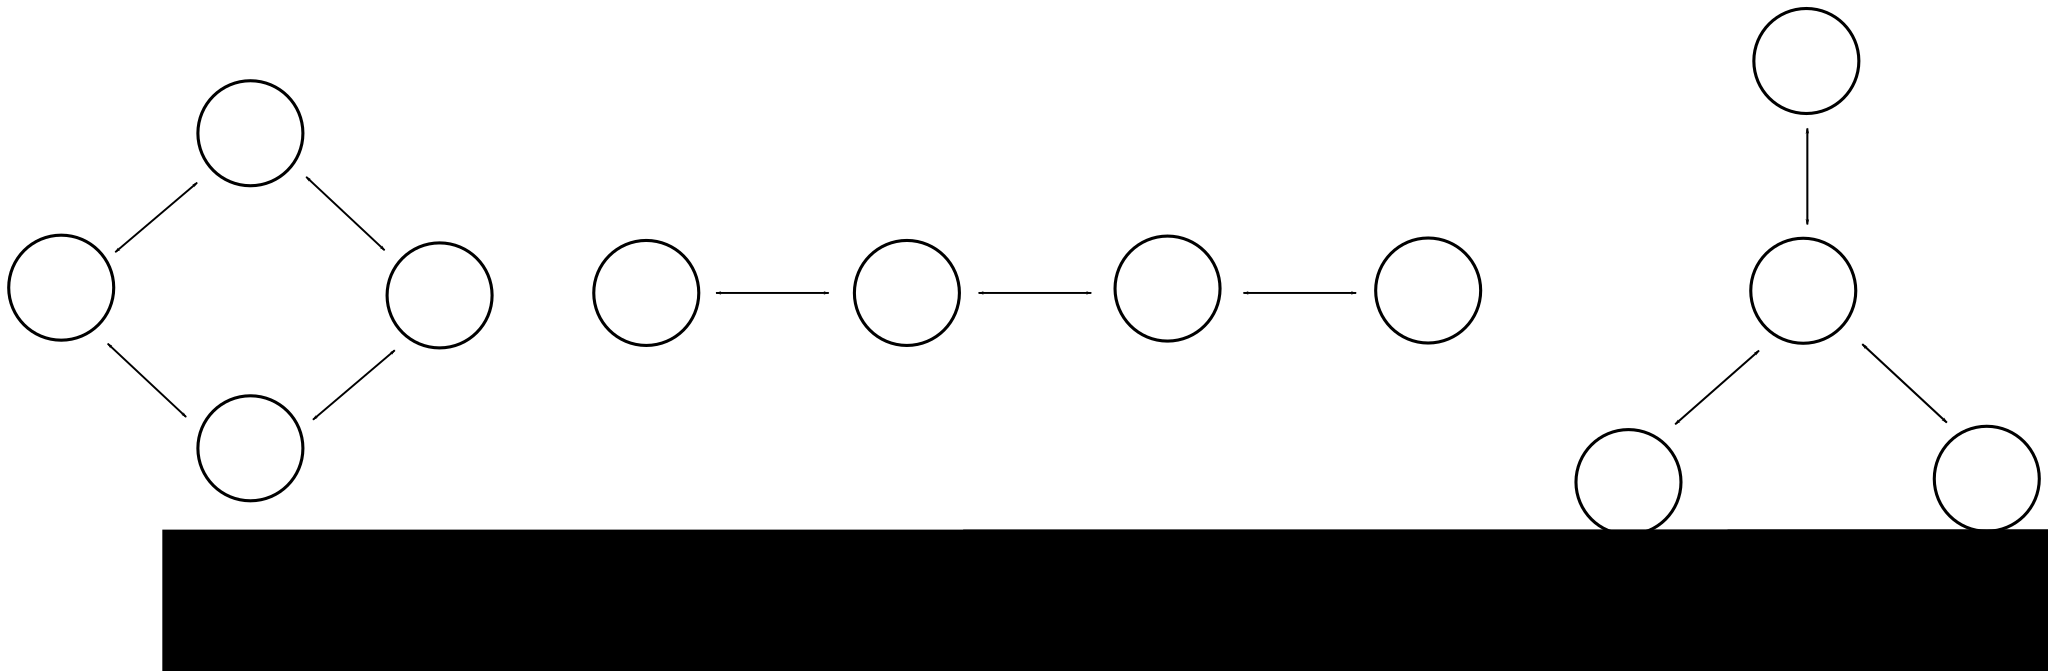
\includegraphics[width=0.45\textwidth]{figures/com_topo}
	\caption{Three types of topologies: (a)circular topology; (b)serial topology; (c)star topology}
	\label{fig:com_topo}
\end{figure}

\subsection{Distributed Bayesian Filter for Multiple Robots}\label{subsec:dbf}
The generic Distributed Bayesian Filter (DBF) is introduced in this section, which was also stated in \cite{hlinka2015distributed} and \cite{furukawa2006recursive}. 
Each robot has its individual estimation of the probability density function (PDF) of target position, called \textit{individual PDF}. 
The $i^\text{th}$ individual PDF at time $k$ is defined as $P^i_{pdf}(x^T_{k-1}|z^i_{1:k-1},z^{\mathcal{Q}_i}_{1:k-1})$. 
Before starting DBF, the individual PDF is initialized by the prior function $P^i_{pdf}(x^T_0|z^i_0,z^{\mathcal{Q}_i}_0)=P(x^T_0)$, given all available prior information including past experience and environmental knowledge. Then the individual PDF is recursively estimated by two steps, i.e., prediction step and updating step, based on the observations of the robots in $\mathcal{Q}_i$.
 
\subsubsection{Prediction}
The $i^\text{th}$ individual PDF at time $k-1$ is known, denoted as $P^i_{pdf}(x^T_{k-1}|z^i_{1:k-1},z^{\mathcal{Q}_i}_{1:k-1})$. 
At time $k$, the prior individual PDF is first predicted forward by using the Chapman-Kolmogorov equation:
\begin{align}\label{eqn:bayes_pred}
&P^i_{pdf}(x^T_k|z^i_{1:k-1},z^{\mathcal{Q}_i}_{1:k-1})\notag\\
&=\int P(x^T_k|x^T_{k-1})P^i_{pdf}(x^T_{k-1}|z^i_{1:k-1},z^{\mathcal{Q}_i}_{1:k-1})dx^T_{k-1}
\end{align}
where $P(x^T_k|x^T_{k-1})$ is a Markov motion model of the target, independent of robot states. 
This model describes the state transition probability of the target from a prior state $x^T_{k-1}$ to posterior state $x^T_k$. 
Note that the target can be static in many search applications, such as the indoor search for stationary objects\cite{kulich2014single}. 
For a static target, its Markov motion model is simplified to be
\begin{equation*}
P(x^T_k|x^T_{k-1})=\begin{cases}
1 & \text{if}\; x^T_k=x^T_{k-1}\\
0 & \text{if}\; x^T_k\neq x^T_{k-1}
\end{cases}
\end{equation*}
and \cref{eqn:bayes_pred} can be reduced to $P^i_{pdf}(x^T_{k}|z^i_{1:k-1},z^{\mathcal{Q}_i}_{1:k-1})=P^i_{pdf}(x^T_{k-1}|z^i_{1:k-1},z^{\mathcal{Q}_i}_{1:k-1})$.

\subsubsection{Updating}
At time step $k$, the $i^\text{th}$ individual PDF is then updated by Bayes' formula using the latest available observations at time $k$: 
\small\begin{align}\label{eqn:bayes_upd}
&P^i_{pdf}(x^T_k|z^i_{1:k},z^{\mathcal{Q}_i}_{1:k})\notag\\
&=K_iP^i_{pdf}(x^T_k|z^i_{1:k-1},z^{\mathcal{Q}_i}_{1:k-1})P(z^i_k|x^T_k)\prod\limits_{j\in\mathcal{Q}_i}P(z^j_k|x^T_k)
\end{align}\normalsize
where $K_i$ is a normalization factor, given by:
\small\begin{align*}
K_i=1/\int P^i_{pdf}(x^T_k|z^i_{1:k-1},z^{\mathcal{Q}_i}_{1:k-1})P(z^i_k|x^T_k)\prod\limits_{j\in\mathcal{Q}_i}P(z^j_k|x^T_k)dx^T_k
\end{align*}\normalsize
where $P^i_{pdf}(x^T_k|z^i_{1:k},z^{\mathcal{Q}_i}_{1:k})$ is called posterior individual PDF; $P(z^i_k|x^T_k)$ is the likelihood function of observation $z^i_k$, described in \cref{eqn:bin_sensor1} and \cref{eqn:bin_sensor0}.

\section{Distributed Bayesian Filter via Local Exchange of Observation}\label{sec:leo-dbf}
This study proposes a Distributed Bayesian Filtering (DBF) algorithm based on LEO strategy, shorted as LEO-DBF. The LEO only uses the local communication within the neighborhood of each robot, but allows to broadcast observations of each robot to any other nodes by multi-hopping along the shortest path in the undirected and connected network. The theoretical analysis show that LEO-DBF can ensure the consistency and consensus of individual PDF  while requiring much less communication burden than any statistics dissemination-based DBFs. 

\subsection{Algorithm for Local Exchange of observations (LEO)}\label{subsec:leo}
Under the LEO, each robot contains a communication buffer (CB) to store its latest knowledge of the observations of all robots: 
\begin{equation*}
\mathbf{z}^i_k=\left[ z^1_{k^i_1},\dots,z^N_{k^i_N}\right]
\end{equation*}
where $z^j_{k^i_j}$ represents the observation made by ${j^\text{th}}$ robot at time $k^i_j$. Note that under LEO, $\mathcal{Q}_i=\left\lbrace 1,\dots,N\right\rbrace $. At time k, $z^j_{k^i_j}$ is received and stored in ${i^\text{th}}$ robot CB, in which $k^i_j$ is the latest available observation time of ${j^\text{th}}$ robot known by ${i^\text{th}}$ robot. Due to the communication delay of multi-hopping, $k^i_j<k$ always holds in practice.\\

The \textbf{LEO algorithm} is stated as follows:

%\begin{tabular}{l}
%\toprule
%LEO Algorithm\\
%\midrule
\textbf{(1) Initialization:} 
The buffer of $i^\text{th}$ robot is initialized when $k=0$: 
\begin{equation*}
%$\begin{array}{c}
	z^j_{k^i_j}=\emptyset,\; k^i_j=0,\;j=1:N
%\end{array}$\\
\end{equation*}

\textbf{(2) Repeat the following steps for i-th robot until stop:}

(2.1) Receiving Step:

The $i^\text{th}$ robot receives all CBs of its neighboring robots. 
The received CBs are totally $|\mathcal{N}_i|$ groups, each of which corresponding to the (k-1)-step CB of a robot in  . 
The received CB from $l^\text{th}$ ($l\in \mathcal{N}_i$) robot is denoted as
\begin{equation*}
\mathbf{z}^l_{k-1}=\left[ z^1_{{k-1}^l_1},\dots,z^N_{{k-1}^l_N}\right],\; l\in\mathcal{N}_i
\end{equation*}

(2.2) Observation Step: 

The $i^\text{th}$ robot updates $z^j_{k^i_j}$ by its own observation at current step:
\begin{equation*}
z^j_{k^i_j}=z^i_k,\;k^i_j=k,\;\text{if }j=i.
\end{equation*}

(2.3) Comparison Step:

The $i^\text{th}$ robot updates other elements of its own CB, i.e., $z^j_{k^i_j},\;j\neq i$, by selecting the latest information among all received CBs from $\mathcal{N}_i$. For all $j\neq i$,
\begin{align*}
l_\text{latest}&=\argmax_{l\in \mathcal{N}_i,i}\left\lbrace\left(k-1\right)^i_j,\left(k-1\right)^l_j  \right\rbrace\\
z^j_{k^i_j}&=z^j_{\left(k-1\right)^{l_\text{latest}}_j},\; k^i_j=\left(k-1\right)^{l_\text{latest}}_j
\end{align*} 

(2.4) Sending Step:

The $i^\text{th}$ robot broadcasts its updated CB to all of its neighbors defined in $\mathcal{N}_i$. $\hfill\blacksquare$\\
%\bottomrule
%\end{tabular}

\begin{figure}%[thpb]
	\centering
	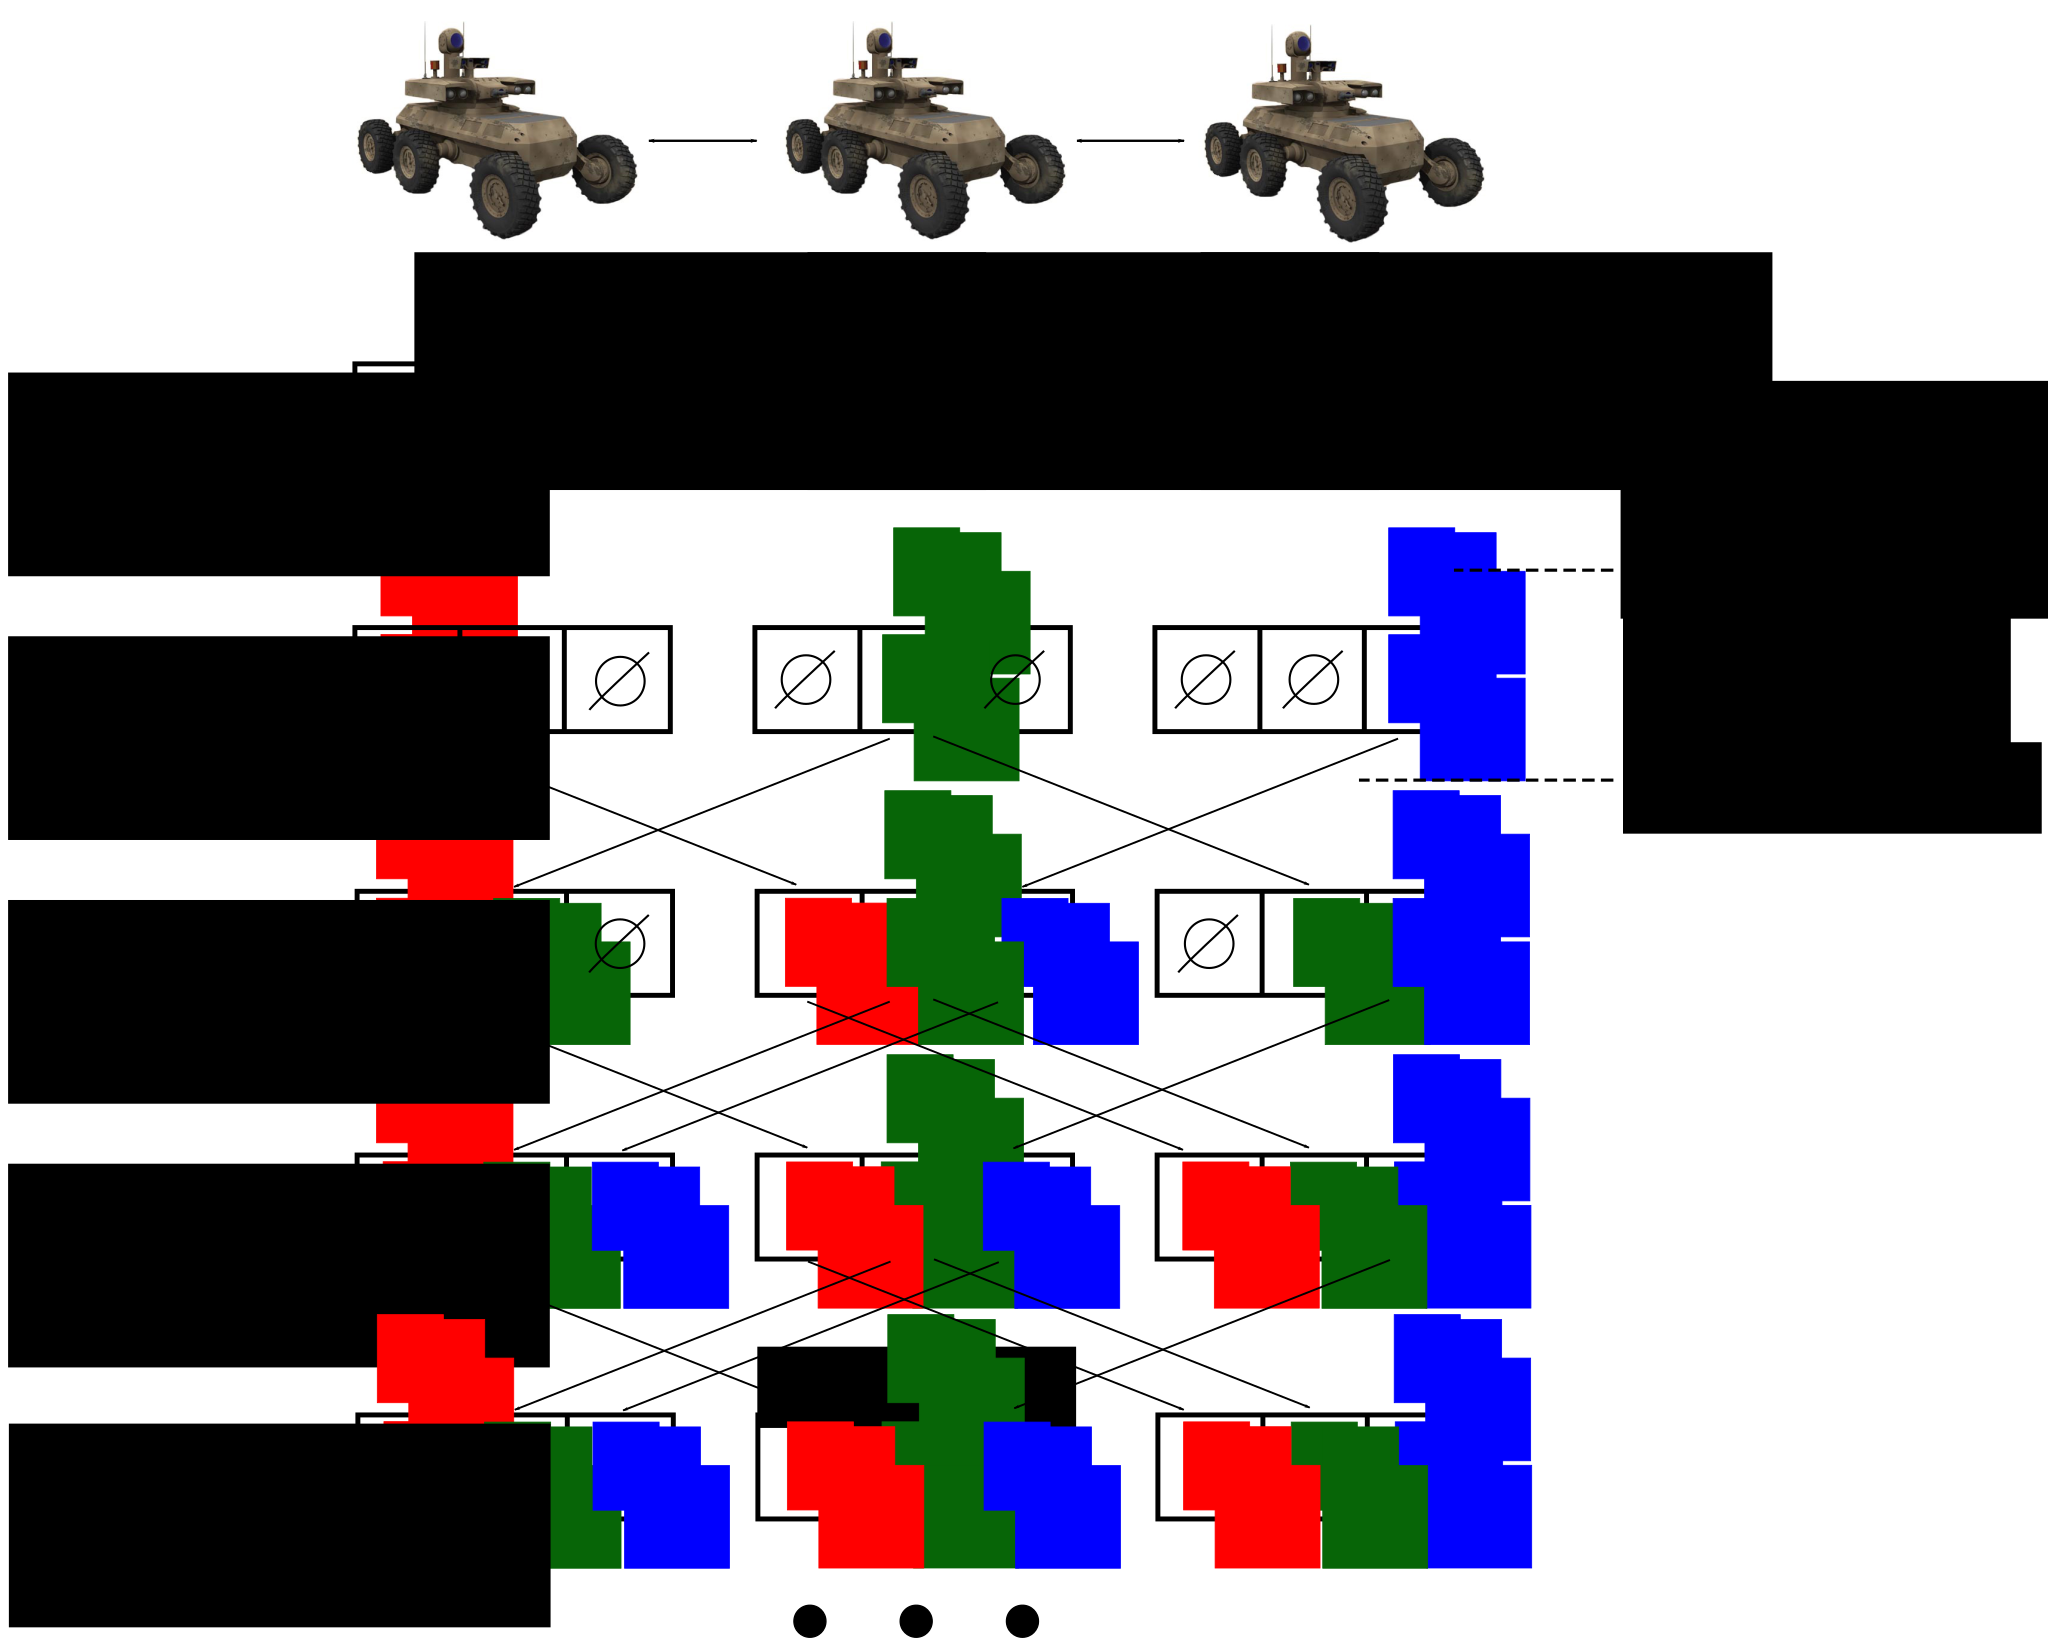
\includegraphics[width=0.45\textwidth]{figures/data_exchange}
	\caption{Example of LEO with three robots using linear communication topology}
	\label{fig:LEO}
\end{figure}

\cref{fig:LEO} illustrates the LEO algorithm with 3 robots using a serial topology. Two facts can be observed in Figure 2: (1) all robot CBs are filled within 3 steps, which means under LEO each robot has a maximum delay of 2 steps when receiving observations from other robots; (2) after filled, the updating of CBs are non-intermittent, which means each robot continuously receives newer observations of other robots. Extending the two facts to a network of N robots, we have the following proposition:

\begin{prop}\label{prop1}
For an undirected and connected network of N robots with fixed topology, LEO uses the shortest path(s) between i and j to exchange observation, i.e., the delay $\tau_{i,j}$ between i and j is equivalent to the length of their shortest path(s). 	
\end{prop}
\begin{proof} 
Without loss of generality, assume that there is a unique shortest path between i and j, denoted by $T^{j,i}_{n^*}=\left(v_1,\dots,v_{n^*}\right)$, with $v_1=j,v_{n^*}=i,v_{m+1}\in\mathcal{N}_{v_m}$. 
Then, the distance between i and j is $d(j,i)=n^*-1$. 
The following mathematical induction will prove \Cref{prop1}.

Step (1): For $d(j,i)=1$, this means $j\in\mathcal{N}_i$ and j can directly send $z^j_k$ to i. Then $z^j_k$ is stored in $i^\text{th}$ CB at time $k+1$, i.e. $\tau_{i,j}=1$. 
\Cref{prop1} holds for $d(j,i)=1,\;i,j\in\left\lbrace 1,\dots,N\right\rbrace $.

Step (2): Suppose that \Cref{prop1} holds for $d(j,i)=s,\;s\geq 2$. 
Then for $d(j,i)=s+1$, i.e., $n^*=s+2$, by the Bellman's principle of optimality, the path $T^{j,l}_{n^*-1}=\left(v_1,\dots,v_{n^*-1}\right)$ is the shortest path between j and l, where $v_{n^*-1}=l$ and $i\in \mathcal{N}_l$. 
The assumption that \Cref{prop1} holds for $d(j,i)=s$ implies that $z^j_k$ is received and stored in $l^\text{th}$ robot's CB at time $k+s$. 
Since $i\in\mathcal{N}_i$, $i^\text{th}$ robot receives $z^j_k$ at $k+s+1$. 
Therefore $\tau_{i,j}=s+1$. 
For any other path $T^{j,i}_{n}=\left(v_1,\dots,v_{n}\right)$ with $n>n^*$, $z^j_k$ cannot be received by $i^\text{th}$ robot at $k+s+1$. 
This proves the \Cref{prop1} for $d(j,i)=s+1$. 
\end{proof}

\begin{cor}\label{cor1}
For the same topology assumption in \Cref{prop1}, all elements in $\mathbf{z}^i_k$ under LEO become filled when $k\geq N$.	
\end{cor}
\begin{proof}
In a network of $N$ robots, the maximal length of shortest paths is no greater than $N-1$. Based on \Cref{prop1}, $\tau_{i,j}\leq N-1$ and thus all elements of $\mathbf{z}^i_k$ become filled when $k\geq N$
\end{proof}

\begin{cor}\label{cor2}
For the same topology in \Cref{prop1}, once all elements in $\mathbf{z}^i_k$ are filled, the updating of each element is non-intermittent. 	
\end{cor}
\begin{proof}
For a network with fixed topology, the shortest path between any nodes is fixed. Based on \Cref{prop1}, $\tau_{i,j}$ is constant, and then the updating of each element in $\mathbf{z}^i_k$ is non-intermittent.
\end{proof}

\begin{rem}
	Compared to statistics dissemination, LEO is a more communication-efficient approach for distributed filtering. 
	To be specific, consider an $M\times M$ grid environment with a network of $N$ robots, the transmitted data of LEO between each pair of robots are only the CB of each robot, the length of which is $O(N)$. 
	On the contrary, the length of transmitted data for a statistics-dissemination approach is $O(M^2)$, which is the size of environment grid. 
	Since $M$ is generally much larger than $N$ in target search and tracking community, LEO requires much less communication resources than the statistics-dissemination approaches.
\end{rem}

\subsection{Algorithm of LEO-DBF for a Static Target}\label{subsec:leo-dbf-sta-tar} 

This section gives the LEO-DBF for a static target. Each robot stores last-step individual PDF, i.e., $(k-1)^\text{th}$ step. The assumption of static target can simplify the Bayesian filter, in which the prediction step is unnecessary. Therefore, the $i^\text{th}$ individual PDF is only updated by 
\begin{equation}\label{eqn:leo-dbf-sta-tar}
P^i_{pdf}(x^T|\mathbf{z}^i_{1:k})=K_iP^i_{pdf}(x^T|\mathbf{z}^i_{1:k-1})\prod\limits_{j=1}^{N}P(z^j_{k^i_j}|x^T)
\end{equation}
where
\begin{equation*}
K_i=1/\int P^i_{pdf}(x^T|\mathbf{z}^i_{1:k-1})\prod\limits_{j=1}^{N}P(z^j_{k^i_j}|x^T)dx^T
\end{equation*}


\subsection{Algorithm of LEO-DBF for a Moving target}\label{subsec:leo-dbf-mov-tar}
This section gives the LEO-DBF for a moving target. 
Instead of storing last-step PDF, each robot maintains an individual PDF for the time step $(k-N)$ and a triangular matrix of history observations from $(k-N+1)^\text{th}$ to $k^\text{th}$ steps. 
The $i^\text{th}$ individual PDF is then alternatively predicted and updated by using aforementioned Bayesian filter (\cref{eqn:bayes_pred} and \cref{eqn:bayes_upd}) from $(k-N)^\text{th}$ to $k^\text{th}$ step.
\cref{fig:LEO-DBF} illustrates the LEO-DBF procedure for the $1^\text{st}$ robot. 

\begin{figure}%[thpb]
	\centering
	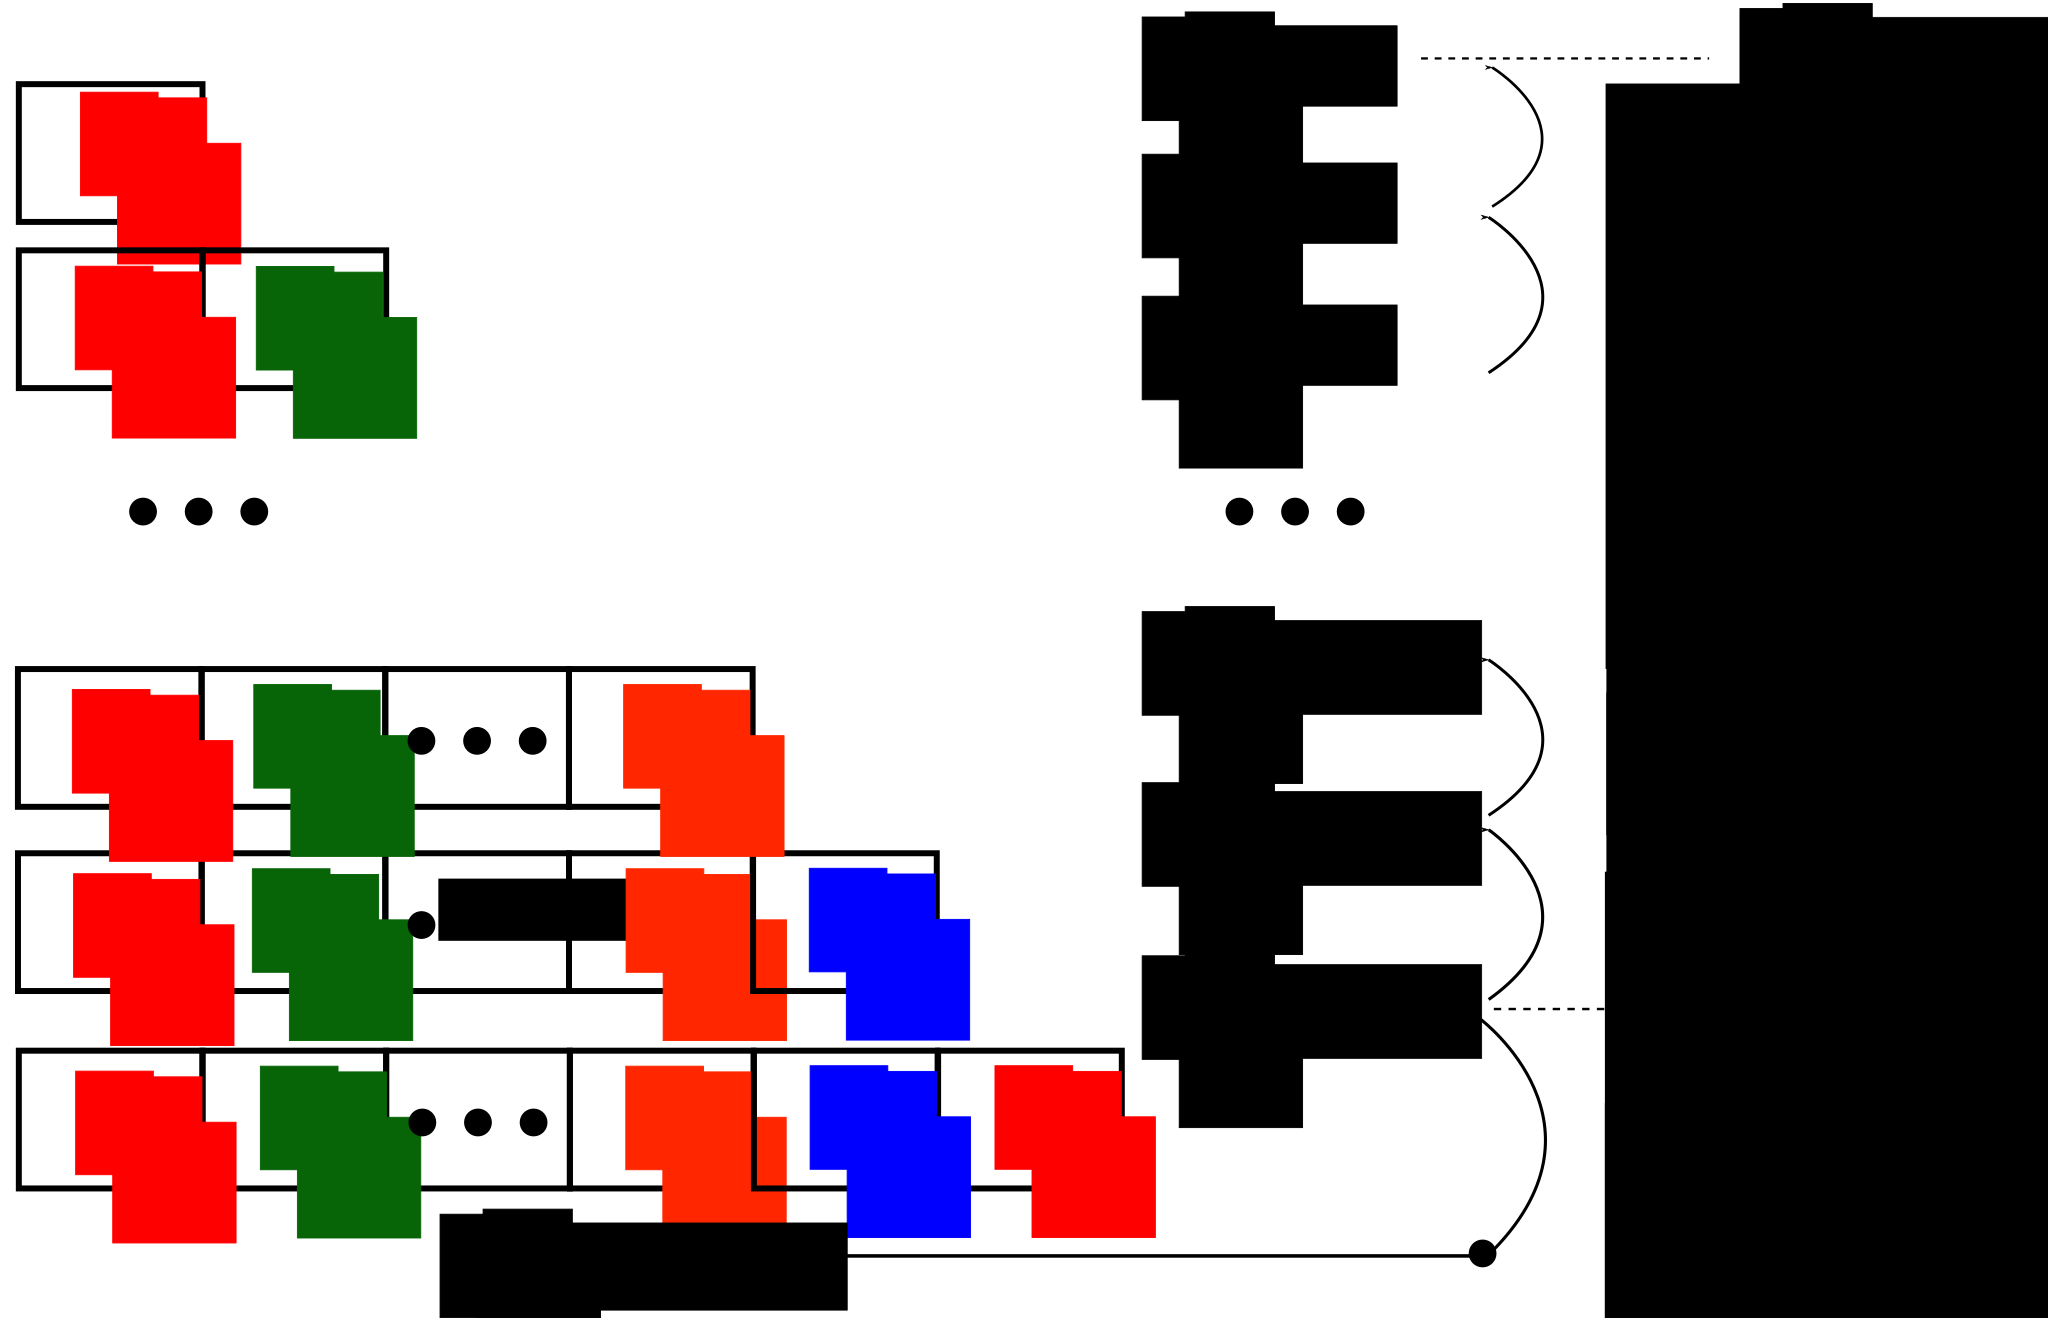
\includegraphics[width=0.45\textwidth]{figures/DBF_demo}
	\caption{Example of LEO-DBF for $1^\text{st}$ robot at time $k$. The current individual PDF is $ P^1_{PDF}(x^T_{k-N}|z^1_{1:k-N},\dots,z^N_{1:k-N})$, denoted as $ P^1_{PDF}(k-N)$ in the figure. The robot first calculates $ P^1_{virt}(k-N+1)$ using DBF and stores it as $ P^1_{PDF}(k-N+1)$. Repeating DBF until obtaining $ P^1_{PDF}(k)$, which is then used as the target PDF estimation of i-th robot}
	\label{fig:LEO-DBF}
\end{figure}

For the $i^\text{th}$ robot at $k^\text{th}$ step, the \textbf{LEO-DBF algorithm} for moving target is:
%\begin{enumerate}

	\textbf{(1)} The stored individual PDF for $(k-N)^\text{th}$ step is:
	\small\begin{equation*}
		P^i_{pdf}(x^T_{k-N}|z^1_{1:k-N},\dots,z^N_{1:k-N})
	\end{equation*}\normalsize
	
	\textbf{(2)} Initialize a virtual PDF by assigning the individual PDF to it:
	\small\begin{equation*}
		P_{virt}(x^T_{k-N})=P^i_{pdf}(x^T_{k-N}|z^1_{1:k-N},\dots,z^N_{1:k-N})
	\end{equation*}\normalsize
		
	\textbf{(3)} From $\xi=1$ to N, repeat two steps of Bayesian filtering:
%	\begin{enumerate}
%		\item 

		(3.1) Prediction 
		\small\begin{align*}
		&P_{virt}^{pre}(x^T_{k-N+\xi})\\=&\int P(x^T_{k-N+\xi}|x^T_{k-N+\xi-1})P_{virt}(x^T_{k-N+\xi-1})dx^T_{k-N+\xi-1}
		\end{align*} \normalsize
				
%		\item 
		(3.2) Updating
		\small\begin{gather*}
		P_{virt}(x^T_{k-N+\xi})=K_\xi P_{virt}^{pre}(x^T_{k-N+\xi})\prod\limits_{j\in\Omega^i_{\xi}}P(z^j_{k_N+\xi}|x^T_{k-N+\xi})\\
		K_\xi=1/\int P_{virt}^{pre}(x^T_{k-N+\xi})\prod\limits_{j\in\Omega^i_{\xi}}P(z^j_{k-N+\xi}|x^T_{k-N+\xi})dx^T_{k-N+\xi}
		\end{gather*} \normalsize
%	\end{enumerate}
	
	\textbf{(4)} Store the first-step virtual PDF as the $(k-N+1)^\text{th}$ individual PDF:
	\begin{equation*}
		P^i_{pdf}(x^T_{k-N+1}|z^1_{1:k-N+1},\dots,z^N_{1:k-N+1})=P_{virt}(x^T_{k-N+1}).
	\end{equation*}
	$\hfill\blacksquare$
	
%\end{enumerate}

%1)	The stored individual PDF for $(k-N)^\text{th}$ step is $ P^i_{pdf}(x^T_{k-N}|z^1_{1:k-N},\dots,z^N_{1:k-N})$.
%
%2)	Initialize a virtual PDF by assigning the individual PDF to it:
%$P_{virt}(x^T_{k-N})=P^i_{pdf}(x^T_{k-N}|z^1_{1:k-N},\dots,z^N_{1:k-N})$
%
%3)	From $\xi=1$ to N, repeat two steps of Bayesian filtering
%(a)	Prediction 
%\begin{align*}
%&P_{virt}^{pre}(x^T_{k-N+\xi})\\=&\int P(x^T_{k-N+\xi}|x^T_{k-N+\xi-1})P_{virt}(x^T_{k-N+\xi-1})dx^T_{k-N+\xi-1}
%\end{align*} 
%(b)	Updating
%\begin{gather*}
%P_{virt}(x^T_{k-N+\xi})=K_\xi P_{virt}^{pre}(x^T_{k-N+\xi})\prod\limits_{j\in\Omega^i_{k-N+\xi}}P(z^j_{k_N+\xi|x^T_{k-N+\xi}})\\
%K_\xi=1/\int P_{virt}^{pre}(x^T_{k-N+\xi})\prod\limits_{j\in\Omega^i_{k-N+\xi}}P(z^j_{k-N+\xi}|x^T_{k-N+\xi})dx^T_{k-N+\xi}
%\end{gather*} 
%  
%4)	Store the first-step virtual PDF as the $(k-N+1)^\text{th}$ individual PDF: $P^i_{pdf}(x^T_{k-N+1}|z^1_{1:k-N+1},\dots,z^N_{1:k-N+1})=P_{virt}(x^T_{k-N+1}).$

Note that $\Omega^i_{\xi}$ denotes the index set of robots whose observation at time $k-N+\xi$ is stored in $i^\text{th}$ robot's CB. 
The target PDF estimation of $i^\text{th}$ robot at current step is $P_{virt}(x^T_k)$.\\

\begin{rem}
	For the static target, each robot only needs current step CB to update individual PDFs. 
	Therefore, except storing individual PDFs, all historical CBs can be discarded and only current-step CB is stored in robot memory, the length of which is $O(N)$. 
	On the contrary, for the moving target, each robot needs to store a triangular matrix of history observation (except current step CB) with $N\times N$ dimension and an $M\times M$ individual PDF, which means that the length of occupied memory in each robot is $O(M^2+N^2)$.
\end{rem}

\section{Proof of Consistency and Consensus}\label{sec:consist_proof}
This section presents a consistency and consensus proof of LEO- DBF. Only the scenarios for the static target are presented, including both static robots and moving robots. The proof for LEO- DBF for moving target is similar to that of static target by assuming that the dynamic model of the target is accurately known, but with more complicated algebraic manipulation. 

Assume that $X^T$ is finite. Define an \textit{equi-parameter} set $X^T_{eq}\subseteq X^T$ such that 
\small\begin{equation*}
P(z_k|x^T_1)=P(z_k|x^T_2),\; \forall x^T_1,x^T_2\in X^T_{eq},\; \forall z_k\in \left\lbrace 0,1\right\rbrace,
\end{equation*}\normalsize
i.e., the probability for generating the same observation $z_k$ is equivalent among sensor models with different parameters in $X^T_{eq}$.
%for any two parameters in $X^T_{eq}$, the sensor model with one of these two parameters generates equivalent probability value for the same observation $z_k$
Since $X^T$ is finite, $X^T_{eq}$ is also finite. 
Let $X^T_{eq,1},\dots,X^T_{eq,u}$ denote all \textit{equi-parameter} sets that partition $X^T$ such that following properties hold:
\begin{enumerate}
	\item $\bigcup^u_{i=1} X^T_{eq,i}= X^T$
	\item $X^T_{eq,i}\cap X^T_{eq,j}=\emptyset,\;i,j\in \left\lbrace 1,\dots,u\right\rbrace ,i\neq j.$
\end{enumerate}
Without loss of generality, assume $x^{T^*}\in X^T_{eq,u}$, where $x^{T^*}$ denotes the actual location of the target. 

\todohere{double check if the following examples for equi-parameter set are accurate}

\begin{rem}
	the \textit{equi-parameter} set depends on the property of the sensor. For example, for a laser scanner with high-fidelity sensing capability, each \textit{equi-parameter} set contains only a small number of target positions.
\end{rem}

\subsection{Proof for static robots}
The consistency of LEO-DBF for static robots is stated as follows: 
\begin{thm}\label{thm:leo-dbf-sta-tar}
	For static robots, each individual PDF by LEO-DBF converges to $ X^T_{eq,1}$ when the number of observations goes to infinity, i.e.
	\begin{equation*}
	P^i_{pdf}(x^T\in X^T_{eq,i}|\mathbf{z}^i_{1:k})\longrightarrow
	\begin{cases}
	1 & \text{if}\; i=1\\
	0 & \text{if}\; i\neq 1
	\end{cases},\;
	k\rightarrow \infty
	\end{equation*}
	where $\mathbf{z}^i_{1:k}=\left(z^1_{1:k_1},\dots,z^N_{1:k_N}\right) $, $\left\lbrace k_1,\dots,k_N\right\rbrace $ are the timestamps of the $i^\text{th}$ robot's latest knowledge of all robots' observations.
\end{thm}

\begin{proof}	
Considering the conditional independence of observations $z^j_k$ for given $x^T\in X^T_{eq,i}$, the batch form of DBF at $k^\text{th}$ step is:
\small\begin{subequations}
	\begin{align*}
		P^i_{pdf}(x^T|\mathbf{z}^i_{1:k})&=P^i_{pdf}(x^T|z^1_{1:k_1},\dots,z^N_{1:k_N})\\
		&=\frac{P^i_{pdf}(x^T)\prod\limits_{j=1}^{N}\prod\limits_{l=1}^{k_j}P(z^j_l|x^T)}{\sum\limits_{x^T\in X^T}\prod\limits_{j=1}^{N}\prod\limits_{l=1}^{k_j}P(z^j_l|x^T)}
	\end{align*}
\end{subequations}\normalsize
\addtocounter{equation}{-1}
where $P^i_{pdf}$ is initial $i^\text{th}$ individual PDF. 
It is known from \Cref{cor1} and \Cref{cor2} that $k-N<k_j\leq k$.\\

Compare $P^i_{pdf}(x^T|\mathbf{z}^i_{1:k})$ with $P^i_{pdf}(x^{T*}|\mathbf{z}^i_{1:k})$:
\small\begin{equation}\label{eqn:cmp}
\frac{P^i_{pdf}(x^T|\mathbf{z}^i_{1:k})}{P^i_{pdf}(x^{T*}|\mathbf{z}^i_{1:k})}=\frac{P^i_{pdf}(x^T)\prod\limits_{j=1}^{N}\prod\limits_{l=1}^{k_j}P(z^j_l|x^T)}{P^i_{pdf}(x^{T*})\prod\limits_{j=1}^{N}\prod\limits_{l=1}^{k_j}P(z^j_l|x^{T*})}
\end{equation}\normalsize
Take the logarithm of \cref{eqn:cmp} and average it over k steps:
\small\begin{equation}\label{eqn:cmp_log}
 \frac{1}{k}\ln\frac{P^i_{pdf}(x^T|\mathbf{z}^i_{1:k})}{P^i_{pdf}(x^{T^*}|\mathbf{z}^i_{1:k})}=\frac{1}{k}\ln\frac{P^i_{pdf}(x^T)}{P^i_{pdf}(x^{T^*})}+\sum\limits_{j=1}^{N}\frac{1}{k}\sum\limits_{l=1}^{k_j}\ln\frac{P(z^j_l|x^T)}{P(z^j_l|x^{T^*})}
\end{equation}\normalsize
Since $P^i_{pdf}(x^T)$ and $P^i_{pdf}(x^{T^*})$ are bounded,
\begin{equation}\label{eqn:cmp_lim1}
\lim\limits_{k\rightarrow \infty}\frac{1}{k}\ln\frac{P^i_{pdf}(x^T)}{P^i_{pdf}(x^{T^*})}\longrightarrow 0
\end{equation}
The binary observations subject to Bernoulli distribution $B(1,p_j)$, yielding
\begin{equation*}
P^i_{pdf}(z^j_k|x^T)=p^{z^j_k}_j(1-p_j)^{1-z^j_k}
\end{equation*}
where $p_j=P(z^j_k=1|x^T)$. Utilizing the fact that (1) $z^j_l$ are conditionally independent samples from $B(1,p_j^*)$ , and (2) $k-N<k_j\leq k$, the law of large numbers yields
\begin{equation*}
\lim\limits_{k\rightarrow \infty}\frac{1}{k}\sum\limits_{l=1}^{k_j}z^j_l=p^*_j,\quad \lim\limits_{k\rightarrow \infty}\frac{1}{k}(k_j-\sum\limits_{l=1}^{k_j}z^j_l)=1-p^*_j
\end{equation*}
where $p_j^*=P(z^j_k=1|x^{T^*})$. Then, 
\small\begin{equation}\label{eqn:cmp_lim2}
\lim\limits_{k\rightarrow \infty}\frac{1}{k}\sum\limits_{l=1}^{k_j}\ln\frac{P(z^j_l|x^T)}{P(z^j_l|x^{T^*})}=p^*_j\ln \frac{p_j}{p^*_j}+(1-p^*_j)\ln \frac{1-p_j}{1-p^*_j}
\end{equation}\normalsize
Note that the right-hand side of \cref{eqn:cmp_lim2} achieves maximum if and only if $p_j=p_j^*$. 
Considering \cref{eqn:cmp_lim1} and \cref{eqn:cmp_lim2}, the limit of \cref{eqn:cmp_log} can be obtained:
\small \begin{equation}\label{eqn:lim}
 \lim\limits_{k\rightarrow \infty}\frac{1}{k}\ln\frac{P^i_{pdf}(x^T|\mathbf{z}^i_{1:k})}{P^i_{pdf}(x^{T^*}|\mathbf{z}^i_{1:k})}=\sum\limits_{j=1}^{N}p^*_j\ln \frac{p_j}{p^*_j}+(1-p^*_j)\ln \frac{1-p_j}{1-p^*_j}
 \end{equation}\normalsize
It is known from \cref{eqn:lim} that
\begin{enumerate}
	\item When $p_j\neq p^*_j$, that is $x^T\notin X^T_{eq,1}$,
	\begin{align*}
		\lim\limits_{k\rightarrow \infty}\frac{1}{k}\ln\frac{P^i_{pdf}(x^T|\mathbf{z}^i_{1:k})}{P^i_{pdf}(x^{T^*}|\mathbf{z}^i_{1:k})} & <0,\;\text{thus }\\
		\lim\limits_{k\rightarrow \infty}\ln\frac{P^i_{pdf}(x^T|\mathbf{z}^i_{1:k})}{P^i_{pdf}(x^{T^*}|\mathbf{z}^i_{1:k})} & =0
	\end{align*}	
	\item When $p_j= p^*_j$, that is $x^T\in X^T_{eq,1}$, \begin{align*}
	\lim\limits_{k\rightarrow \infty}\frac{1}{k}\ln\frac{P^i_{pdf}(x^T|\mathbf{z}^i_{1:k})}{P^i_{pdf}(x^{T^*}|\mathbf{z}^i_{1:k})} & =0,\;\text{thus }\\
	\lim\limits_{k\rightarrow \infty}\ln\frac{P^i_{pdf}(x^T|\mathbf{z}^i_{1:k})}{P^i_{pdf}(x^{T^*}|\mathbf{z}^i_{1:k})} & =1
	\end{align*}
\end{enumerate}
\end{proof}


\subsection{Proof for moving sensors}
\todohere{complete this sentence}
The difficulty for moving robots lies on ****. The main idea is to classify the states etc. . Before stating main theorem, the following lemma is introduced:
\begin{lem}\label{lem1}
	For a set of robots with a collection of finite possible states $Y^R$, there exists at least one state for each robot that it visits for infinite times as k tends to infinity.
\end{lem}

\begin{proof}
Let $n^{i,k}_j$ denote the times that $i^\text{th}$ robot visits $j^\text{th}$ state in $Y^R$ up to time $k$. Then, $\sum\limits_{j} n^{i,k}_j=k$. It is straightforward to see that $\exists n^{i,k}_j,$ such that $n^{i,k}_j\rightarrow \infty,$ as $k\rightarrow \infty$.
\end{proof}

The consistency of LEO-DBF for moving robots is stated as follows:
\begin{thm}\label{thm:leo-dbf-mov-tar}
	Under the condition of moving robots, each individual PDF by LEO-DBF converges to $X^T_{eq,1}$ when the number of observations goes to infinity, i.e.,
	\begin{equation*}
		P^i_{pdf}(x^T\in X^T_{eq,i}|\mathbf{z}^i_{1:k})\longrightarrow
		\begin{cases}
		1 & \text{if}\; i=1\\
		0 & \text{if}\; i\neq 1
		\end{cases},\;
		k\rightarrow \infty
	\end{equation*}
	where $\mathbf{z}^i_{1:k}=(z^1_{1:k_1},\dots,z^N_{1:k_N})$, $\left\lbrace k_1,\dots,k_N\right\rbrace$ are the timestamps of $i^\text{th}$ robot?s latest knowledge of all robots? observations.
\end{thm}

\begin{proof}
Let $M\subseteq\left\lbrace 1,\dots,k_j\right\rbrace\times Y^R $ denote the set of (time, position) pairs to indicate $j^\text{th}$ robot?s state at the corresponding time of observation.

Similar to \Cref{thm:leo-dbf-sta-tar}, the batch form of DBF at $k^\text{th}$ step is:
\small\begin{equation}\label{eqn:cmp2}
\frac{P^i_{pdf}(x^T|\mathbf{z}^i_{1:k})}{P^i_{pdf}(x^{T^{*}}|\mathbf{z}^i_{1:k})}=\frac{P^i_{pdf}(x^T)\prod\limits_{j=1}^{N}\prod\limits_{l\in M^i}P(z^j_l|x^T)}{P^i_{pdf}(x^{T^{*}})\prod\limits_{j=1}^{N}\prod\limits_{l\in M^i}P(z^j_l|x^{T^{*}})}
\end{equation}\normalsize
The only difference is that $P(z^j_l|X^T)$ needs to be grouped according to the robot state. 
For each robot, there exists at least one state from which the robot obtains infinite observations as $k\rightarrow \infty$, according to \Cref{lem1}. 
We can classify all the states into finite-observation states and infinite-observation states. 
For the former, it is straightforward to know that their contribution to \cref{eqn:lim} is zero.
Therefore, the proof of \cref{eqn:cmp2} can be reduced to infinite-observation states, which is similar to \Cref{thm:leo-dbf-sta-tar}.
\end{proof}

\begin{rem}
	Since $X^T_{eq,1}$ is unique, the consistency of LEO-DBF means the consensus of individual PDFs.
\end{rem}

\begin{rem}
	The consistency property differentiates LEO-DBF from the statistics dissemination-based filtering approaches. 
	In fact, the statistics dissemination-based methods can ensure the convergence of the state estimate among robots. 
	However, there's no guarantee whether the agreed estimate is close to the true target position.
\end{rem}

\section{Simulation}\label{sec:sim}
This section simulates three searching scenarios in order to demonstrate the effectiveness of LEO-BDF. In all scenarios, six robots are utilized and each robot is equipped with a binary sensor. All sensors are modeled with identical Gaussian functions:
\small\begin{align*}
P(z=1|x^T;x^s)&=\exp\left\lbrace -\frac{1}{2}(x^T-x^s)^T{\Sigma}^{-1}(x^T-x^s)\right\rbrace \\
P(z=0|x^T;x^s)&=1-P(z=1|x^T;x^s)
\end{align*}\normalsize
where $x^s$ denotes the robot position where current observation is obtained. 
%Figure 4 shows the 1-D illustration of Gaussian binary sensor model.

The first scenario consists of six static robots and single static target, which acts as a proof of concept of the LEO strategy for static target case. 
The second scenario subsequently deals with six moving robots for searching the single static target. Robot positions are randomly generated at each time step. 
The third scenario is presented that contains six moving sensors and one moving target. 
A single-integrator dynamics is used for the target motion model.

\subsection{Static Robots, Static Target}\label{subsec:sim1}

The positions of six static robots are shown as stars in \cref{fig:sta_sen_sta_tar1}.
Each robot constantly receives binary observations of the target.
LEO-DBF \cref{eqn:leo-dbf-sta-tar} is implemented on each robot for target position estimation.

\cref{fig:sta_sen_sta_tar} shows the estimation results of the static target. 
After the initial observation, each sensor forms a circular individual PDF, centered at the corresponding sensor position. 
As more observations are received, the posterior individual PDF concentrates on the true location of the target. 
\cref{fig:entropy} (a) shows the decrease of the entropy of the posterior distribution, indicating the uncertainty reduction of the estimated target position.

\begin{figure}%[thpb]
	\centering
	\begin{subfigure}[b]{0.23\textwidth}
		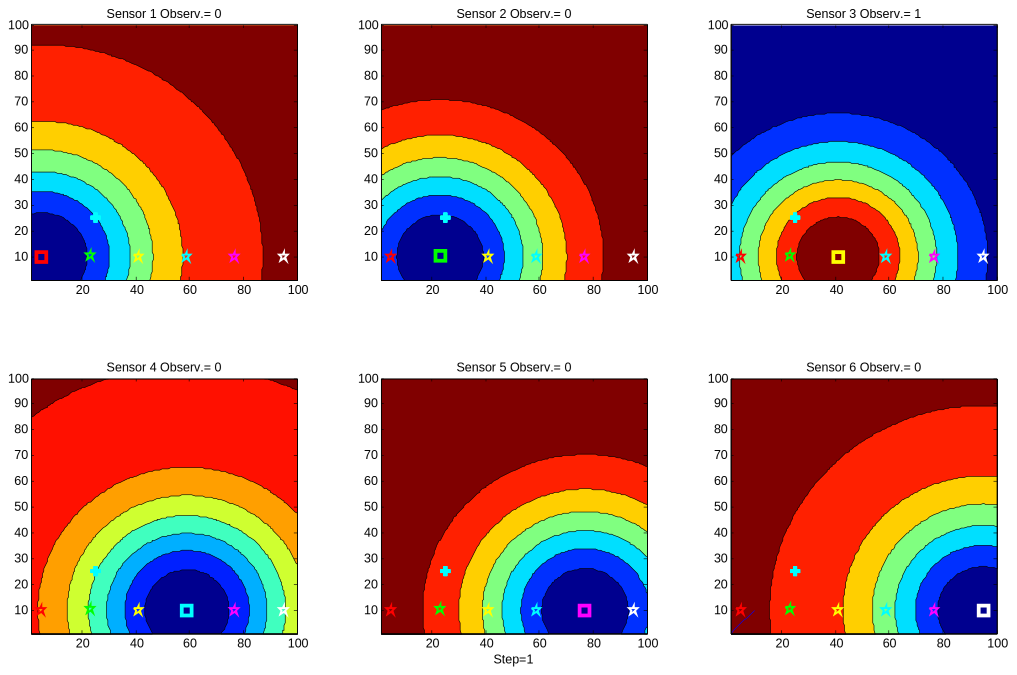
\includegraphics[width=\textwidth]{figures/sta_sen_sta_tar_1}
		\caption{Step 1}\label{fig:sta_sen_sta_tar1}
	\end{subfigure}
	~
	\begin{subfigure}[b]{0.23\textwidth}
		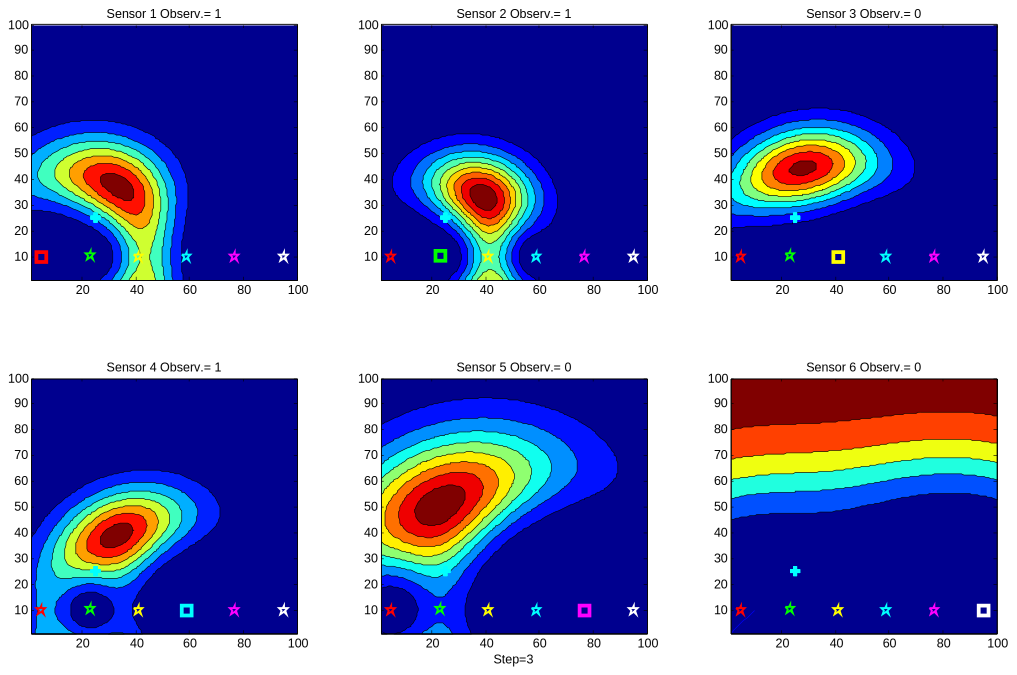
\includegraphics[width=\textwidth]{figures/sta_sen_sta_tar_3}
		\caption{Step 3}\label{fig:sta_sen_sta_tar2}
	\end{subfigure}
	~
	\begin{subfigure}[b]{0.23\textwidth}
		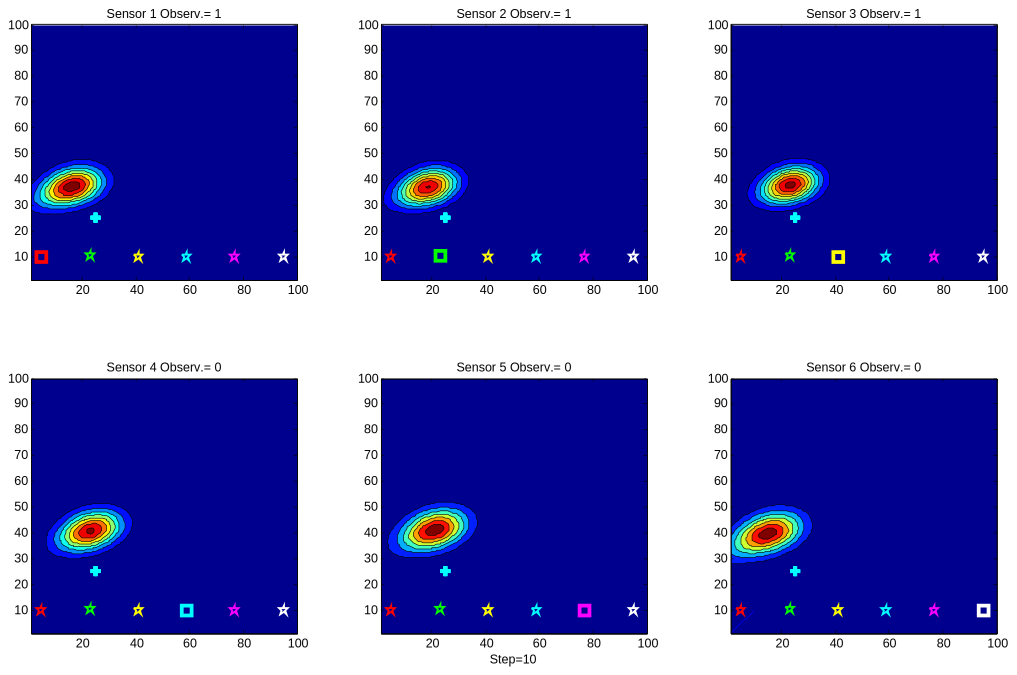
\includegraphics[width=\textwidth]{figures/sta_sen_sta_tar_10}
		\caption{Step 10}\label{fig:sta_sen_sta_tar3}
	\end{subfigure}
	~
	\begin{subfigure}[b]{0.23\textwidth}
		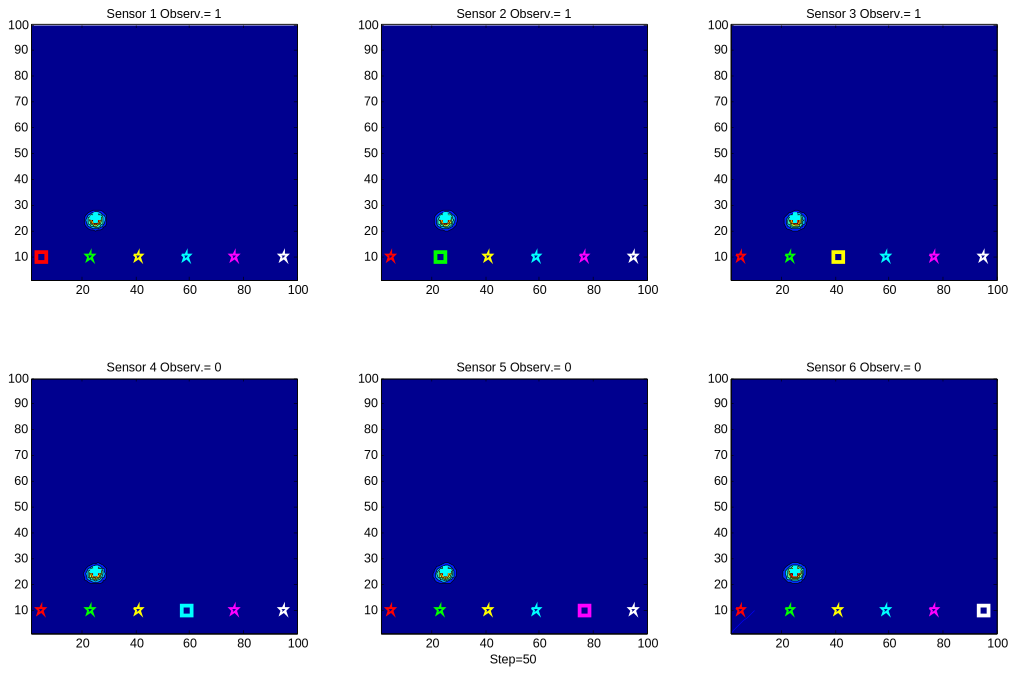
\includegraphics[width=\textwidth]{figures/sta_sen_sta_tar_50}
		\caption{Step 50}\label{fig:sta_sen_sta_tar4}
	\end{subfigure}
	\caption{Static robots' individual PDFs of the static target.}
	\label{fig:sta_sen_sta_tar}
\end{figure}

\subsection{Moving Robots, Static Target}
The six robots move within the field to estimate the target position. 
The motion planning of robots for effective target search has received much attention in the past years. 
In this work, the robot positions are randomly generated at each time in order to demonstrate the effectiveness of the LEO-DBF approach. 
Readers interested in robot motion planning can refer to \cite{tisdale2009autonomous,furukawa2006recursive}.

\cref{fig:mov_sen_sta_tar} shows the estimation results over time. 
Similar to the results in \cref{subsec:sim1}, the posterior individual PDF concentrates to the true target location. 
\cref{fig:entropy} (b) shows the decrease of the entropy of the posterior distribution.

\begin{figure}%[thpb]
	\centering
	\begin{subfigure}[b]{0.23\textwidth}
		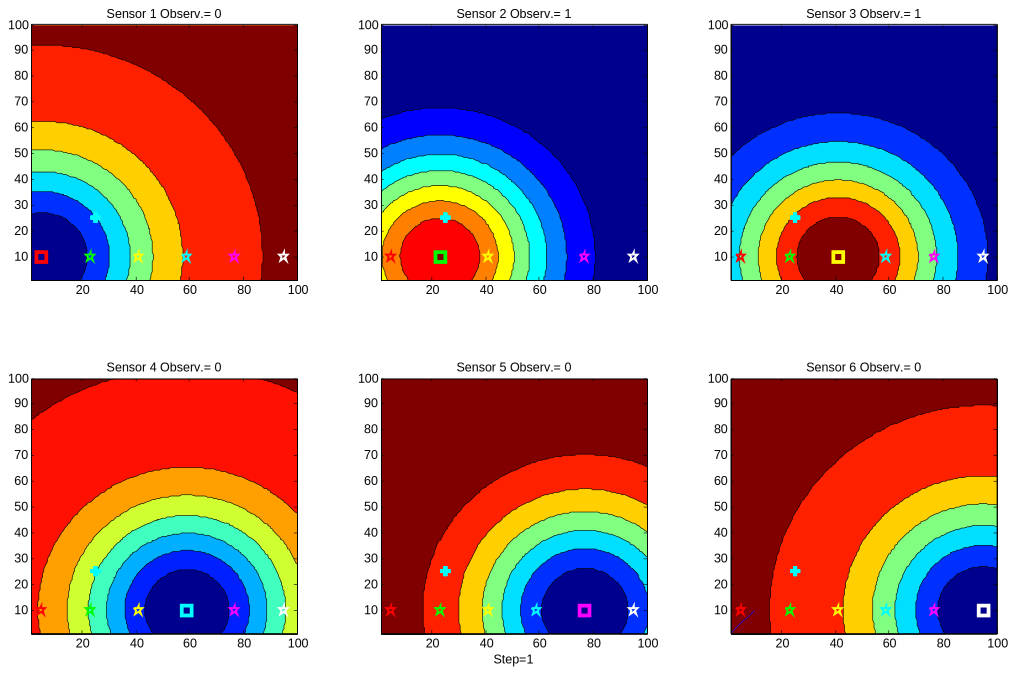
\includegraphics[width=\textwidth]{figures/mov_sen_sta_tar_1}
		\caption{Step 1}\label{fig:mov_sen_sta_tar1}
	\end{subfigure}
	~
	\begin{subfigure}[b]{0.23\textwidth}
		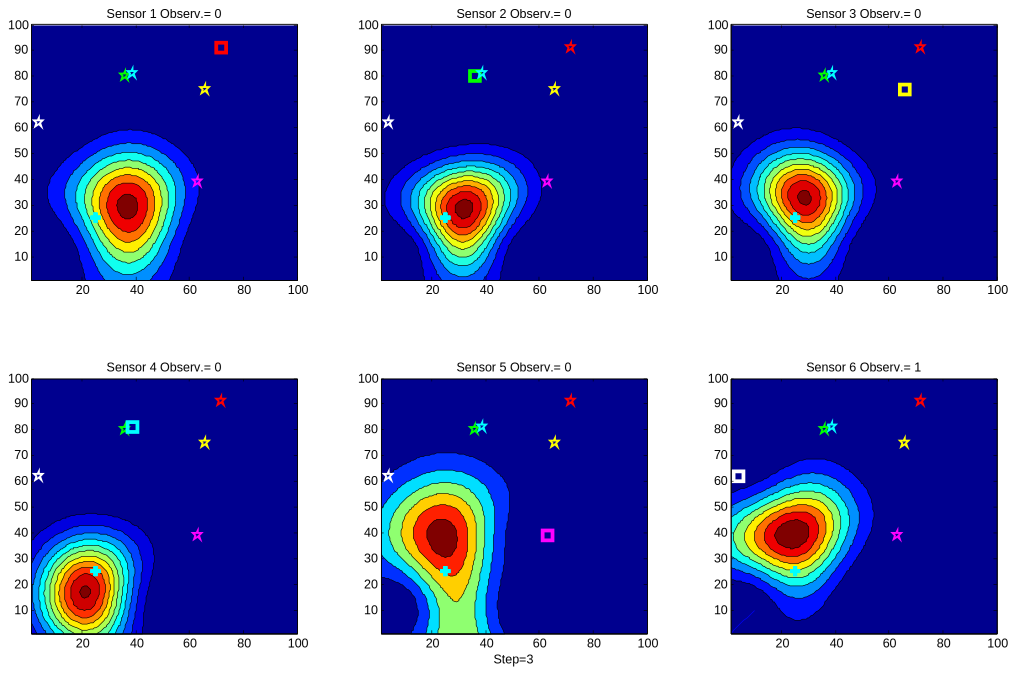
\includegraphics[width=\textwidth]{figures/mov_sen_sta_tar_3}
		\caption{Step 3}\label{fig:mov_sen_sta_tar2}
	\end{subfigure}
	~
	\begin{subfigure}[b]{0.23\textwidth}
		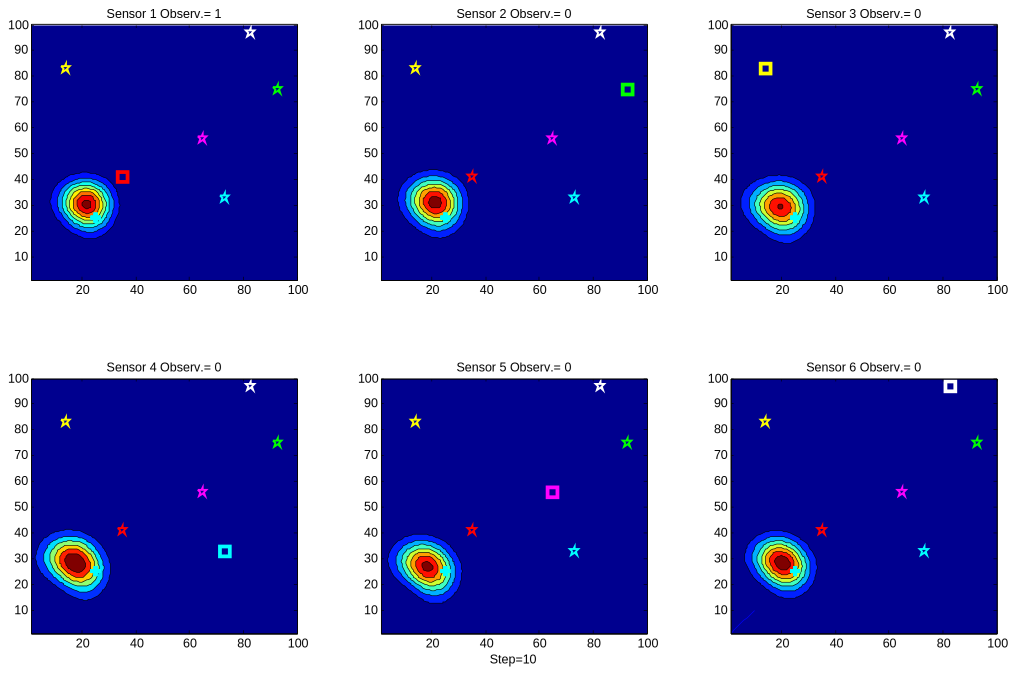
\includegraphics[width=\textwidth]{figures/mov_sen_sta_tar_10}
		\caption{Step 10}\label{fig:mov_sen_sta_tar3}
	\end{subfigure}
	~
	\begin{subfigure}[b]{0.23\textwidth}
		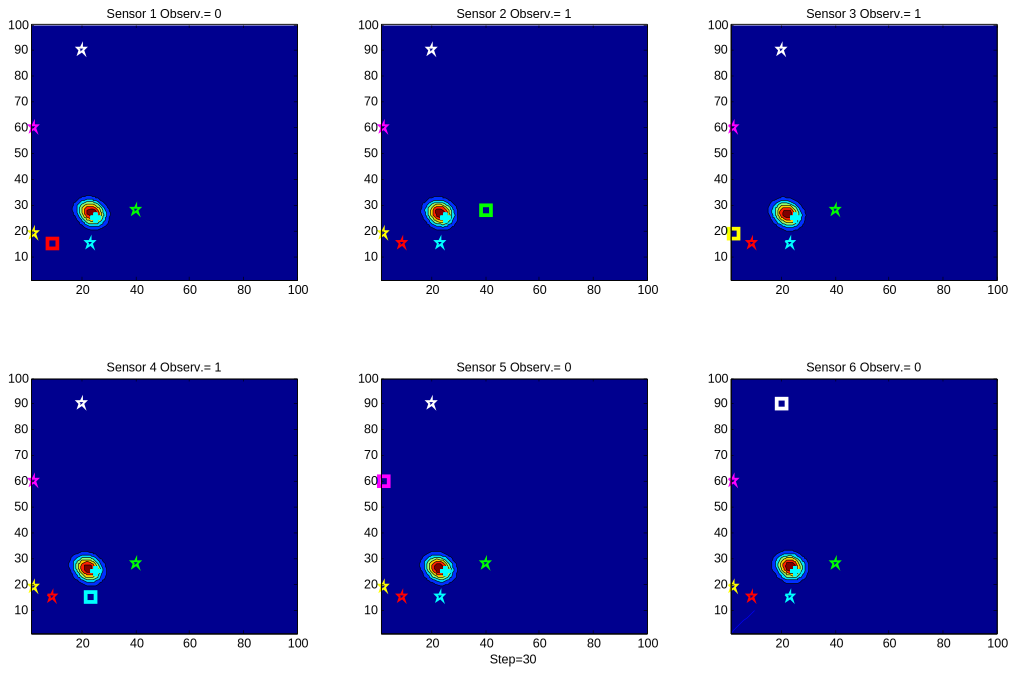
\includegraphics[width=\textwidth]{figures/mov_sen_sta_tar_30}
		\caption{Step 30}\label{fig:mov_sen_sta_tar4}
	\end{subfigure}
	\caption{Moving robots' individual PDFs of the static target.}
	\label{fig:mov_sen_sta_tar}
\end{figure}

\subsection{Moving Robots, Moving Target}
The target in this scenario moves on the horizontal plane and the dynamics is given by a single-integrator model:
\begin{equation*}
x^T(k+1)=x^T(k)+v
\end{equation*}
where $v$ is the constant velocity of the target.

The LEO-DBF described in \cref{subsec:leo-dbf-mov-tar} is used as the distributed Bayesian filters.
\cref{fig:mov_sen_mov_tar} shows the estimation results of the moving target. 
It can be noticed that similar to the case of static target, the posterior individual PDFs concentrate to the true target location at each time, even when the target constantly moves.
\cref{fig:entropy} (c) shows the decrease of the entropy of the posterior distribution.

\begin{figure}%[thpb]
	\centering
	\begin{subfigure}[b]{0.23\textwidth}
		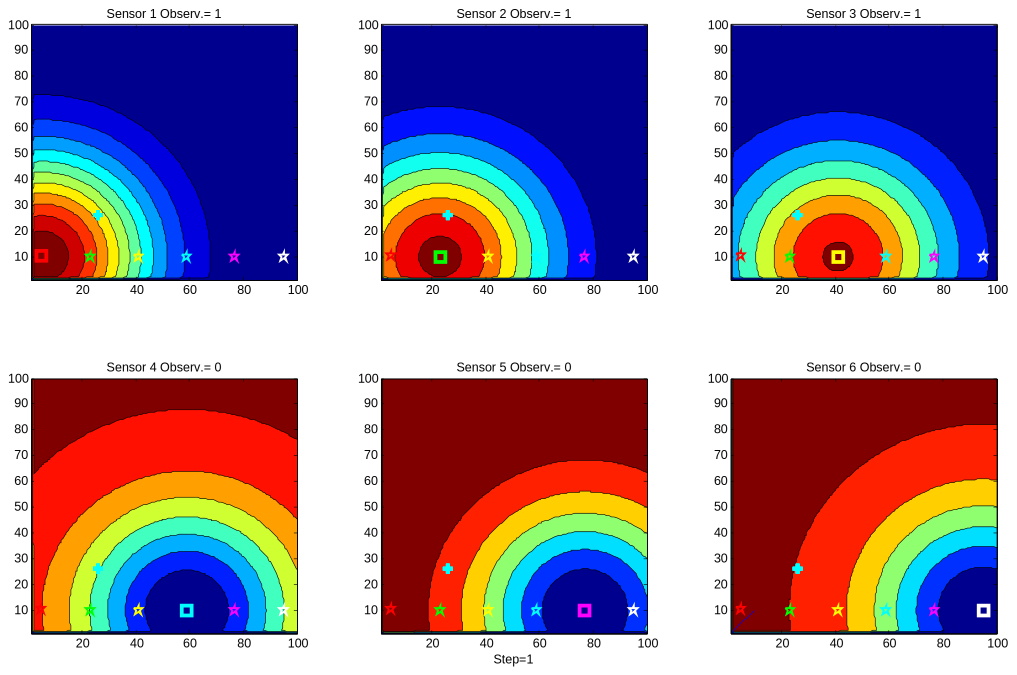
\includegraphics[width=\textwidth]{figures/mov_sen_mov_tar_1}
		\caption{Step 1}\label{fig:mov_sen_mov_tar1}
	\end{subfigure}
	~
	\begin{subfigure}[b]{0.23\textwidth}
		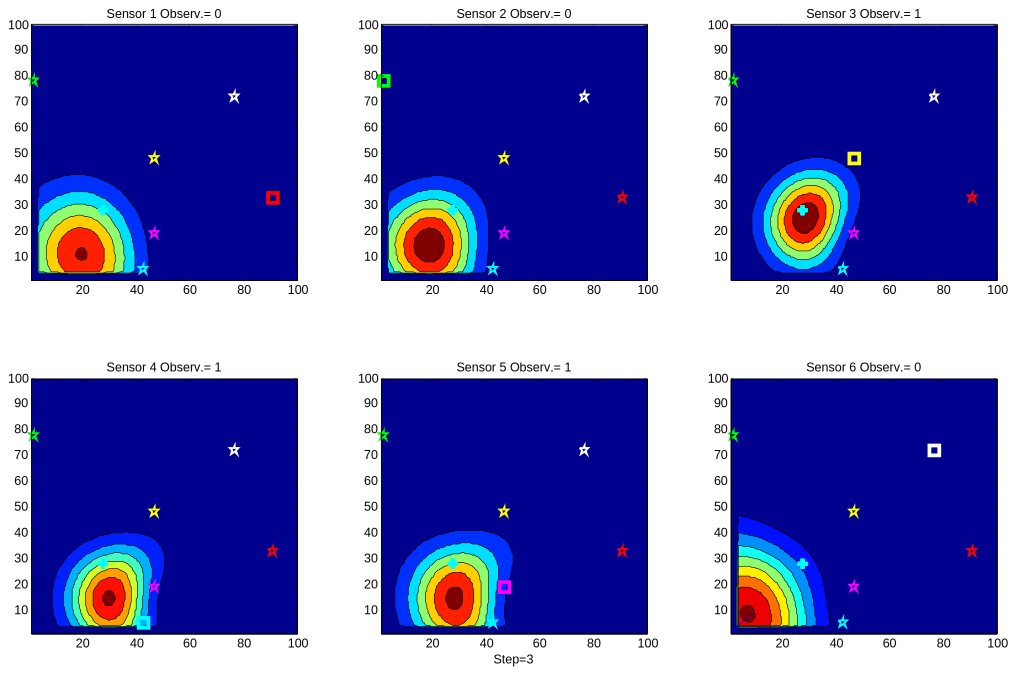
\includegraphics[width=\textwidth]{figures/mov_sen_mov_tar_3}
		\caption{Step 3}\label{fig:mov_sen_mov_tar2}
	\end{subfigure}	
	~
	\begin{subfigure}[b]{0.23\textwidth}
		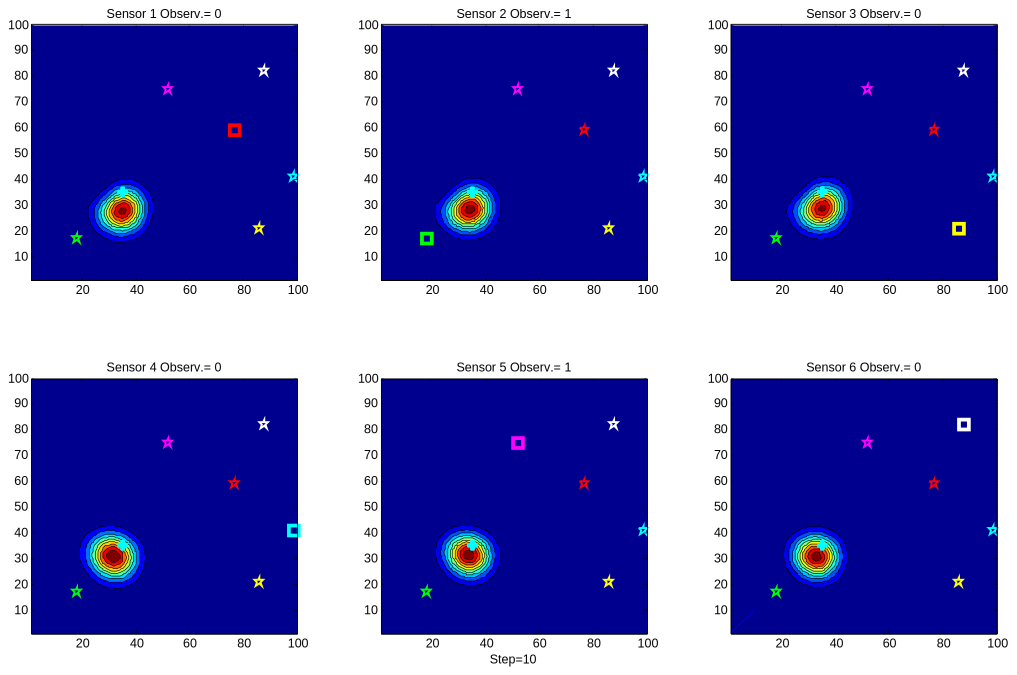
\includegraphics[width=\textwidth]{figures/mov_sen_mov_tar_10}
		\caption{Step 10}\label{fig:mov_sen_mov_tar3}
	\end{subfigure}	
	~
	\begin{subfigure}[b]{0.23\textwidth}
		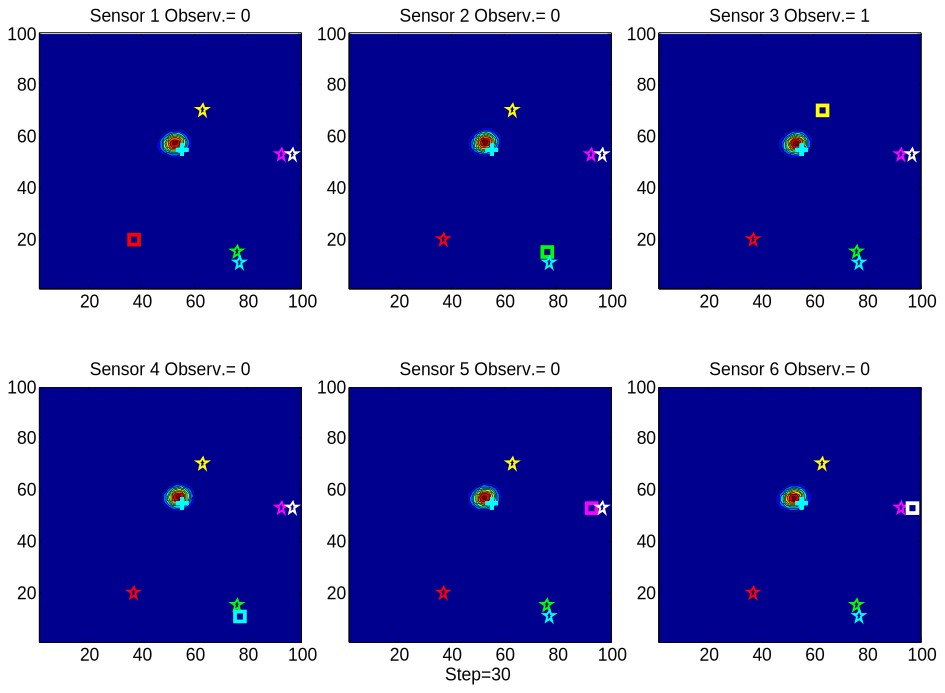
\includegraphics[width=\textwidth]{figures/mov_sen_mov_tar_30}
		\caption{Step 30}\label{fig:mov_sen_mov_tar4}
	\end{subfigure}
	\caption{Moving robots' individual PDFs of the moving target.}
	\label{fig:mov_sen_mov_tar}
\end{figure}

\begin{figure}%[thpb]
	\centering
	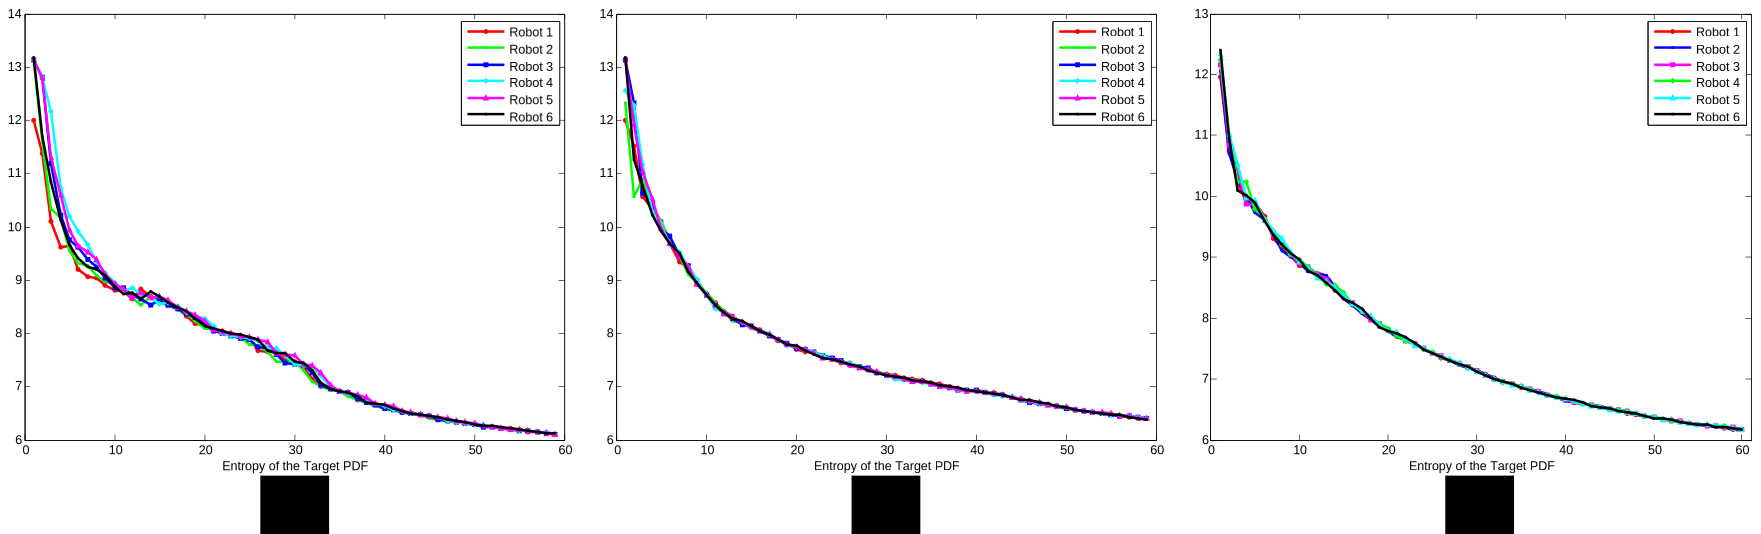
\includegraphics[width=0.5\textwidth]{figures/entropy}
	\caption{Entropy of individual PDFs over time: (a) static robots and static target; (b) moving robots and static target; (c) moving robots and moving target.}
	\label{fig:entropy}
\end{figure}

\section{CONCLUSION}\label{sec:conclu}
In this study, we proposed the local-exchange-of-observation (LEO) strategy for distributed Bayesian filters (LEO-DBF) in a multi-robot network with the application of distributed estimation of target position in the environment. 
With fixed communication topology, LEO guarantees the spread of all robots' observations within the network.
Once elements in communication buffer (CB) gets filled, each robot can received and update its CB non-intermittently under LEO.
Two LEO-DBFs are proposed for estimating the position of the static and the moving target, respectively. 
For the static target, each robot locally fuses the latest knowledge of all robots' observations by only considering the updating step of the Bayesian filter. 
For the moving target, a triangle matrix of historical observations is maintained by each robot. 
Upon obtaining the latest available observations of all robots, an iterative Bayesian filtering procedure is applied that alternates between prediction and updating steps. 
The consistency of LEO-DBF is proved by showing the asymptotic concentration of posterior individual PDF to the \textit{equi-parameter set} containing the actual state, ensuring the agreement between robots' state estimate using LEO-DBF and the actual environment state 
Simulations demonstrated the effectiveness of LEO-DBF for tracking both static and moving target.

Future work may include several extensions to the proposed LEO-DBF. LEO under switching topology can leads to unpredictable delay and intermittent transmission. Therefore consensus analysis of individual PDFs requires further analysis. In addition, combining LEO-DBF with robot motion planning is promising for more effective estimation of target state in the environment.

\addtolength{\textheight}{-12cm}   % This command serves to balance the column lengths
                                  % on the last page of the document manually. It shortens
                                  % the textheight of the last page by a suitable amount.
                                  % This command does not take effect until the next page
                                  % so it should come on the page before the last. Make
                                  % sure that you do not shorten the textheight too much.

%%%%%%%%%%%%%%%%%%%%%%%%%%%%%%%%%%%%%%%%%%%%%%%%%%%%%%%%%%%%%%%%%%%%%%%%%%%%%%%%



%%%%%%%%%%%%%%%%%%%%%%%%%%%%%%%%%%%%%%%%%%%%%%%%%%%%%%%%%%%%%%%%%%%%%%%%%%%%%%%%



%%%%%%%%%%%%%%%%%%%%%%%%%%%%%%%%%%%%%%%%%%%%%%%%%%%%%%%%%%%%%%%%%%%%%%%%%%%%%%%%
%\section*{APPENDIX}
%
%Appendixes should appear before the acknowledgment.

%\section*{ACKNOWLEDGMENT}
%
%The preferred spelling of the word �acknowledgment� in America is without an �e� after the �g�. Avoid the stilted expression, �One of us (R. B. G.) thanks . . .�  Instead, try �R. B. G. thanks�. Put sponsor acknowledgments in the unnumbered footnote on the first page.



%%%%%%%%%%%%%%%%%%%%%%%%%%%%%%%%%%%%%%%%%%%%%%%%%%%%%%%%%%%%%%%%%%%%%%%%%%%%%%%%
\bibliographystyle{IEEEtran}
\bibliography{references}

\end{document}
